\documentclass[twoside]{book}

% Packages required by doxygen
\usepackage{fixltx2e}
\usepackage{calc}
\usepackage{doxygen}
\usepackage[export]{adjustbox} % also loads graphicx
\usepackage{graphicx}
\usepackage[utf8]{inputenc}
\usepackage{makeidx}
\usepackage{multicol}
\usepackage{multirow}
\PassOptionsToPackage{warn}{textcomp}
\usepackage{textcomp}
\usepackage[nointegrals]{wasysym}
\usepackage[table]{xcolor}

% Font selection
\usepackage[T1]{fontenc}
\usepackage[scaled=.90]{helvet}
\usepackage{courier}
\usepackage{amssymb}
\usepackage{sectsty}
\renewcommand{\familydefault}{\sfdefault}
\allsectionsfont{%
  \fontseries{bc}\selectfont%
  \color{darkgray}%
}
\renewcommand{\DoxyLabelFont}{%
  \fontseries{bc}\selectfont%
  \color{darkgray}%
}
\newcommand{\+}{\discretionary{\mbox{\scriptsize$\hookleftarrow$}}{}{}}

% Page & text layout
\usepackage{geometry}
\geometry{%
  a4paper,%
  top=2.5cm,%
  bottom=2.5cm,%
  left=2.5cm,%
  right=2.5cm%
}
\tolerance=750
\hfuzz=15pt
\hbadness=750
\setlength{\emergencystretch}{15pt}
\setlength{\parindent}{0cm}
\setlength{\parskip}{3ex plus 2ex minus 2ex}
\makeatletter
\renewcommand{\paragraph}{%
  \@startsection{paragraph}{4}{0ex}{-1.0ex}{1.0ex}{%
    \normalfont\normalsize\bfseries\SS@parafont%
  }%
}
\renewcommand{\subparagraph}{%
  \@startsection{subparagraph}{5}{0ex}{-1.0ex}{1.0ex}{%
    \normalfont\normalsize\bfseries\SS@subparafont%
  }%
}
\makeatother

% Headers & footers
\usepackage{fancyhdr}
\pagestyle{fancyplain}
\fancyhead[LE]{\fancyplain{}{\bfseries\thepage}}
\fancyhead[CE]{\fancyplain{}{}}
\fancyhead[RE]{\fancyplain{}{\bfseries\leftmark}}
\fancyhead[LO]{\fancyplain{}{\bfseries\rightmark}}
\fancyhead[CO]{\fancyplain{}{}}
\fancyhead[RO]{\fancyplain{}{\bfseries\thepage}}
\fancyfoot[LE]{\fancyplain{}{}}
\fancyfoot[CE]{\fancyplain{}{}}
\fancyfoot[RE]{\fancyplain{}{\bfseries\scriptsize Generated by Doxygen }}
\fancyfoot[LO]{\fancyplain{}{\bfseries\scriptsize Generated by Doxygen }}
\fancyfoot[CO]{\fancyplain{}{}}
\fancyfoot[RO]{\fancyplain{}{}}
\renewcommand{\footrulewidth}{0.4pt}
\renewcommand{\chaptermark}[1]{%
  \markboth{#1}{}%
}
\renewcommand{\sectionmark}[1]{%
  \markright{\thesection\ #1}%
}

% Indices & bibliography
\usepackage{natbib}
\usepackage[titles]{tocloft}
\setcounter{tocdepth}{3}
\setcounter{secnumdepth}{5}
\makeindex

% Hyperlinks (required, but should be loaded last)
\usepackage{ifpdf}
\ifpdf
  \usepackage[pdftex,pagebackref=true]{hyperref}
\else
  \usepackage[ps2pdf,pagebackref=true]{hyperref}
\fi
\hypersetup{%
  colorlinks=true,%
  linkcolor=blue,%
  citecolor=blue,%
  unicode%
}

% Custom commands
\newcommand{\clearemptydoublepage}{%
  \newpage{\pagestyle{empty}\cleardoublepage}%
}

\usepackage{caption}
\captionsetup{labelsep=space,justification=centering,font={bf},singlelinecheck=off,skip=4pt,position=top}

%===== C O N T E N T S =====

\begin{document}

% Titlepage & ToC
\hypersetup{pageanchor=false,
             bookmarksnumbered=true,
             pdfencoding=unicode
            }
\pagenumbering{roman}
\begin{titlepage}
\vspace*{7cm}
\begin{center}%
{\Large Chess }\\
\vspace*{1cm}
{\large Generated by Doxygen 1.8.11}\\
\end{center}
\end{titlepage}
\clearemptydoublepage
\tableofcontents
\clearemptydoublepage
\pagenumbering{arabic}
\hypersetup{pageanchor=true}

%--- Begin generated contents ---
\chapter{Chess}
\label{md_README}
\hypertarget{md_README}{}
This is an easy-\/to-\/use chess library. 
\chapter{Hierarchical Index}
\section{Class Hierarchy}
This inheritance list is sorted roughly, but not completely, alphabetically\+:\begin{DoxyCompactList}
\item \contentsline{section}{edu.\+xwei12.\+chess.\+Board$<$ B extends Board$<$ B, C, C extends Coordinates$<$ C $>$}{\pageref{interfaceedu_1_1xwei12_1_1chess_1_1_board}}{}
\item \contentsline{section}{edu.\+xwei12.\+chess.\+Board$<$ Rectangle\+Board, Rectangle\+Position $>$}{\pageref{interfaceedu_1_1xwei12_1_1chess_1_1_board}}{}
\begin{DoxyCompactList}
\item \contentsline{section}{edu.\+xwei12.\+chess.\+Rectangle\+Board}{\pageref{classedu_1_1xwei12_1_1chess_1_1_rectangle_board}}{}
\end{DoxyCompactList}
\item \contentsline{section}{edu.\+xwei12.\+chess.\+Coordinates$<$ T extends Coordinates$<$ T $>$}{\pageref{interfaceedu_1_1xwei12_1_1chess_1_1_coordinates}}{}
\item \contentsline{section}{edu.\+xwei12.\+chess.\+Coordinates$<$ Rectangle\+Position $>$}{\pageref{interfaceedu_1_1xwei12_1_1chess_1_1_coordinates}}{}
\begin{DoxyCompactList}
\item \contentsline{section}{edu.\+xwei12.\+chess.\+Rectangle\+Position}{\pageref{classedu_1_1xwei12_1_1chess_1_1_rectangle_position}}{}
\end{DoxyCompactList}
\item \contentsline{section}{edu.\+xwei12.\+chess.\+Default\+Piece}{\pageref{enumedu_1_1xwei12_1_1chess_1_1_default_piece}}{}
\item \contentsline{section}{edu.\+xwei12.\+chess.\+Extended\+Piece}{\pageref{enumedu_1_1xwei12_1_1chess_1_1_extended_piece}}{}
\item \contentsline{section}{edu.\+xwei12.\+chess.\+Game$<$ B extends Board$<$ B, C, C extends Coordinates$<$ C $>$}{\pageref{classedu_1_1xwei12_1_1chess_1_1_game}}{}
\item \contentsline{section}{edu.\+xwei12.\+chess.\+Game$<$ Rectangle\+Board, Rectangle\+Position $>$}{\pageref{classedu_1_1xwei12_1_1chess_1_1_game}}{}
\begin{DoxyCompactList}
\item \contentsline{section}{edu.\+xwei12.\+chess.\+Standard\+Game}{\pageref{classedu_1_1xwei12_1_1chess_1_1_standard_game}}{}
\end{DoxyCompactList}
\item \contentsline{section}{edu.\+xwei12.\+chess.\+Game\+Observer$<$ B extends Board$<$ B, C, C extends Coordinates$<$ C $>$}{\pageref{interfaceedu_1_1xwei12_1_1chess_1_1_game_observer}}{}
\item \contentsline{section}{edu.\+xwei12.\+chess.\+Game\+Observer$<$ B, C $>$}{\pageref{interfaceedu_1_1xwei12_1_1chess_1_1_game_observer}}{}
\item \contentsline{section}{edu.\+xwei12.\+chess.\+Game\+Observer$<$ Rectangle\+Board, Rectangle\+Position $>$}{\pageref{interfaceedu_1_1xwei12_1_1chess_1_1_game_observer}}{}
\begin{DoxyCompactList}
\item \contentsline{section}{edu.\+xwei12.\+chess.\+Game\+Test}{\pageref{classedu_1_1xwei12_1_1chess_1_1_game_test}}{}
\item \contentsline{section}{edu.\+xwei12.\+chess.\+gui.\+App\+Controller}{\pageref{classedu_1_1xwei12_1_1chess_1_1gui_1_1_app_controller}}{}
\end{DoxyCompactList}
\item \contentsline{section}{edu.\+xwei12.\+chess.\+gui.\+G\+U\+I\+Test}{\pageref{classedu_1_1xwei12_1_1chess_1_1gui_1_1_g_u_i_test}}{}
\item \contentsline{section}{edu.\+xwei12.\+chess.\+Game$<$ B extends Board$<$ B, C, C extends Coordinates$<$ C $>$.Move}{\pageref{classedu_1_1xwei12_1_1chess_1_1_game_1_1_move}}{}
\item \contentsline{section}{edu.\+xwei12.\+chess.\+Piece$<$ B extends Board, C extends Coordinates$<$ C $>$}{\pageref{classedu_1_1xwei12_1_1chess_1_1_piece}}{}
\item \contentsline{section}{edu.\+xwei12.\+chess.\+Piece$<$ edu.\+xwei12.\+chess.\+Rectangle\+Board, edu.\+xwei12.\+chess.\+Rectangle\+Position $>$}{\pageref{classedu_1_1xwei12_1_1chess_1_1_piece}}{}
\item \contentsline{section}{edu.\+xwei12.\+chess.\+Game$<$ B extends Board$<$ B, C, C extends Coordinates$<$ C $>$.State}{\pageref{enumedu_1_1xwei12_1_1chess_1_1_game_1_1_state}}{}
\item Application\begin{DoxyCompactList}
\item \contentsline{section}{edu.\+xwei12.\+chess.\+gui.\+App\+Controller}{\pageref{classedu_1_1xwei12_1_1chess_1_1gui_1_1_app_controller}}{}
\end{DoxyCompactList}
\item Test\+Case\begin{DoxyCompactList}
\item \contentsline{section}{edu.\+xwei12.\+chess.\+Game\+Test}{\pageref{classedu_1_1xwei12_1_1chess_1_1_game_test}}{}
\item \contentsline{section}{edu.\+xwei12.\+chess.\+Piece\+Test}{\pageref{classedu_1_1xwei12_1_1chess_1_1_piece_test}}{}
\end{DoxyCompactList}
\end{DoxyCompactList}

\chapter{Class Index}
\section{Class List}
Here are the classes, structs, unions and interfaces with brief descriptions\+:\begin{DoxyCompactList}
\item\contentsline{section}{\hyperlink{classedu_1_1xwei12_1_1chess_1_1gui_1_1_app_controller}{edu.\+xwei12.\+chess.\+gui.\+App\+Controller} }{\pageref{classedu_1_1xwei12_1_1chess_1_1gui_1_1_app_controller}}{}
\item\contentsline{section}{\hyperlink{interfaceedu_1_1xwei12_1_1chess_1_1_board}{edu.\+xwei12.\+chess.\+Board$<$ B extends Board$<$ B, C, C extends Coordinates$<$ C $>$} }{\pageref{interfaceedu_1_1xwei12_1_1chess_1_1_board}}{}
\item\contentsline{section}{\hyperlink{interfaceedu_1_1xwei12_1_1chess_1_1_coordinates}{edu.\+xwei12.\+chess.\+Coordinates$<$ T extends Coordinates$<$ T $>$} }{\pageref{interfaceedu_1_1xwei12_1_1chess_1_1_coordinates}}{}
\item\contentsline{section}{\hyperlink{enumedu_1_1xwei12_1_1chess_1_1_default_piece}{edu.\+xwei12.\+chess.\+Default\+Piece} }{\pageref{enumedu_1_1xwei12_1_1chess_1_1_default_piece}}{}
\item\contentsline{section}{\hyperlink{enumedu_1_1xwei12_1_1chess_1_1_extended_piece}{edu.\+xwei12.\+chess.\+Extended\+Piece} }{\pageref{enumedu_1_1xwei12_1_1chess_1_1_extended_piece}}{}
\item\contentsline{section}{\hyperlink{classedu_1_1xwei12_1_1chess_1_1_game}{edu.\+xwei12.\+chess.\+Game$<$ B extends Board$<$ B, C, C extends Coordinates$<$ C $>$} }{\pageref{classedu_1_1xwei12_1_1chess_1_1_game}}{}
\item\contentsline{section}{\hyperlink{interfaceedu_1_1xwei12_1_1chess_1_1_game_observer}{edu.\+xwei12.\+chess.\+Game\+Observer$<$ B extends Board$<$ B, C, C extends Coordinates$<$ C $>$} }{\pageref{interfaceedu_1_1xwei12_1_1chess_1_1_game_observer}}{}
\item\contentsline{section}{\hyperlink{classedu_1_1xwei12_1_1chess_1_1_game_test}{edu.\+xwei12.\+chess.\+Game\+Test} }{\pageref{classedu_1_1xwei12_1_1chess_1_1_game_test}}{}
\item\contentsline{section}{\hyperlink{classedu_1_1xwei12_1_1chess_1_1gui_1_1_g_u_i_test}{edu.\+xwei12.\+chess.\+gui.\+G\+U\+I\+Test} }{\pageref{classedu_1_1xwei12_1_1chess_1_1gui_1_1_g_u_i_test}}{}
\item\contentsline{section}{\hyperlink{classedu_1_1xwei12_1_1chess_1_1_game_1_1_move}{edu.\+xwei12.\+chess.\+Game$<$ B extends Board$<$ B, C, C extends Coordinates$<$ C $>$.\+Move} }{\pageref{classedu_1_1xwei12_1_1chess_1_1_game_1_1_move}}{}
\item\contentsline{section}{\hyperlink{classedu_1_1xwei12_1_1chess_1_1_piece}{edu.\+xwei12.\+chess.\+Piece$<$ B extends Board, C extends Coordinates$<$ C $>$} }{\pageref{classedu_1_1xwei12_1_1chess_1_1_piece}}{}
\item\contentsline{section}{\hyperlink{classedu_1_1xwei12_1_1chess_1_1_piece_test}{edu.\+xwei12.\+chess.\+Piece\+Test} }{\pageref{classedu_1_1xwei12_1_1chess_1_1_piece_test}}{}
\item\contentsline{section}{\hyperlink{classedu_1_1xwei12_1_1chess_1_1_rectangle_board}{edu.\+xwei12.\+chess.\+Rectangle\+Board} }{\pageref{classedu_1_1xwei12_1_1chess_1_1_rectangle_board}}{}
\item\contentsline{section}{\hyperlink{classedu_1_1xwei12_1_1chess_1_1_rectangle_position}{edu.\+xwei12.\+chess.\+Rectangle\+Position} }{\pageref{classedu_1_1xwei12_1_1chess_1_1_rectangle_position}}{}
\item\contentsline{section}{\hyperlink{classedu_1_1xwei12_1_1chess_1_1_standard_game}{edu.\+xwei12.\+chess.\+Standard\+Game} }{\pageref{classedu_1_1xwei12_1_1chess_1_1_standard_game}}{}
\item\contentsline{section}{\hyperlink{enumedu_1_1xwei12_1_1chess_1_1_game_1_1_state}{edu.\+xwei12.\+chess.\+Game$<$ B extends Board$<$ B, C, C extends Coordinates$<$ C $>$.\+State} }{\pageref{enumedu_1_1xwei12_1_1chess_1_1_game_1_1_state}}{}
\end{DoxyCompactList}

\chapter{Class Documentation}
\hypertarget{classedu_1_1xwei12_1_1chess_1_1gui_1_1_app_controller}{}\section{edu.\+xwei12.\+chess.\+gui.\+App\+Controller Class Reference}
\label{classedu_1_1xwei12_1_1chess_1_1gui_1_1_app_controller}\index{edu.\+xwei12.\+chess.\+gui.\+App\+Controller@{edu.\+xwei12.\+chess.\+gui.\+App\+Controller}}
Inheritance diagram for edu.\+xwei12.\+chess.\+gui.\+App\+Controller\+:\begin{figure}[H]
\begin{center}
\leavevmode
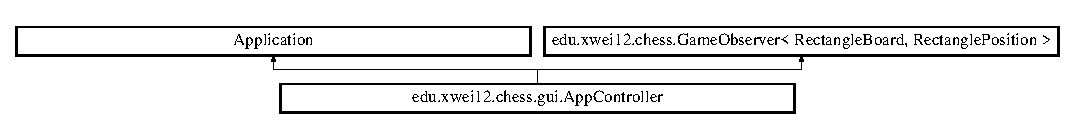
\includegraphics[height=1.290323cm]{classedu_1_1xwei12_1_1chess_1_1gui_1_1_app_controller}
\end{center}
\end{figure}
\subsection*{Public Member Functions}
\begin{DoxyCompactItemize}
\item 
\hyperlink{classedu_1_1xwei12_1_1chess_1_1gui_1_1_app_controller_abceb1198f2298df21da0add550da15e9}{App\+Controller} ()
\item 
void \hyperlink{classedu_1_1xwei12_1_1chess_1_1gui_1_1_app_controller_ac4e307711931ef3465cb0c096c68e301}{start} (Stage primary\+Stage)
\item 
void \hyperlink{classedu_1_1xwei12_1_1chess_1_1gui_1_1_app_controller_a8195eeec526afaa9e3b7e3a3f1cd84b8}{on\+Chess\+Game\+State\+Update} (\hyperlink{classedu_1_1xwei12_1_1chess_1_1_game}{Game} game, \hyperlink{classedu_1_1xwei12_1_1chess_1_1_game_1_1_move}{Game.\+Move} move)
\item 
Image \hyperlink{classedu_1_1xwei12_1_1chess_1_1gui_1_1_app_controller_ab9418c923ea97a7e04d0d148b198be82}{snapshot} ()
\end{DoxyCompactItemize}
\subsection*{Static Public Member Functions}
\begin{DoxyCompactItemize}
\item 
static void {\bfseries main} (String\mbox{[}$\,$\mbox{]} args)\hypertarget{classedu_1_1xwei12_1_1chess_1_1gui_1_1_app_controller_a7d2c18ab0a7334e57bcf937bd5618e76}{}\label{classedu_1_1xwei12_1_1chess_1_1gui_1_1_app_controller_a7d2c18ab0a7334e57bcf937bd5618e76}

\end{DoxyCompactItemize}


\subsection{Detailed Description}
G\+UI demo \begin{DoxyAuthor}{Author}
Xinran Wei 
\end{DoxyAuthor}


\subsection{Constructor \& Destructor Documentation}
\index{edu\+::xwei12\+::chess\+::gui\+::\+App\+Controller@{edu\+::xwei12\+::chess\+::gui\+::\+App\+Controller}!App\+Controller@{App\+Controller}}
\index{App\+Controller@{App\+Controller}!edu\+::xwei12\+::chess\+::gui\+::\+App\+Controller@{edu\+::xwei12\+::chess\+::gui\+::\+App\+Controller}}
\subsubsection[{\texorpdfstring{App\+Controller()}{AppController()}}]{\setlength{\rightskip}{0pt plus 5cm}edu.\+xwei12.\+chess.\+gui.\+App\+Controller.\+App\+Controller (
\begin{DoxyParamCaption}
{}
\end{DoxyParamCaption}
)\hspace{0.3cm}{\ttfamily [inline]}}\hypertarget{classedu_1_1xwei12_1_1chess_1_1gui_1_1_app_controller_abceb1198f2298df21da0add550da15e9}{}\label{classedu_1_1xwei12_1_1chess_1_1gui_1_1_app_controller_abceb1198f2298df21da0add550da15e9}
Constructor\+: initializes a game with G\+UI 

\subsection{Member Function Documentation}
\index{edu\+::xwei12\+::chess\+::gui\+::\+App\+Controller@{edu\+::xwei12\+::chess\+::gui\+::\+App\+Controller}!on\+Chess\+Game\+State\+Update@{on\+Chess\+Game\+State\+Update}}
\index{on\+Chess\+Game\+State\+Update@{on\+Chess\+Game\+State\+Update}!edu\+::xwei12\+::chess\+::gui\+::\+App\+Controller@{edu\+::xwei12\+::chess\+::gui\+::\+App\+Controller}}
\subsubsection[{\texorpdfstring{on\+Chess\+Game\+State\+Update(\+Game game, Game.\+Move move)}{onChessGameStateUpdate(Game game, Game.Move move)}}]{\setlength{\rightskip}{0pt plus 5cm}void edu.\+xwei12.\+chess.\+gui.\+App\+Controller.\+on\+Chess\+Game\+State\+Update (
\begin{DoxyParamCaption}
\item[{{\bf Game}}]{game, }
\item[{{\bf Game.\+Move}}]{move}
\end{DoxyParamCaption}
)\hspace{0.3cm}{\ttfamily [inline]}}\hypertarget{classedu_1_1xwei12_1_1chess_1_1gui_1_1_app_controller_a8195eeec526afaa9e3b7e3a3f1cd84b8}{}\label{classedu_1_1xwei12_1_1chess_1_1gui_1_1_app_controller_a8195eeec526afaa9e3b7e3a3f1cd84b8}
\hyperlink{classedu_1_1xwei12_1_1chess_1_1_game}{Game} state delegate. To update the view after a move. 
\begin{DoxyParams}{Parameters}
{\em game} & game instance \\
\hline
{\em move} & move \\
\hline
\end{DoxyParams}
\index{edu\+::xwei12\+::chess\+::gui\+::\+App\+Controller@{edu\+::xwei12\+::chess\+::gui\+::\+App\+Controller}!snapshot@{snapshot}}
\index{snapshot@{snapshot}!edu\+::xwei12\+::chess\+::gui\+::\+App\+Controller@{edu\+::xwei12\+::chess\+::gui\+::\+App\+Controller}}
\subsubsection[{\texorpdfstring{snapshot()}{snapshot()}}]{\setlength{\rightskip}{0pt plus 5cm}Image edu.\+xwei12.\+chess.\+gui.\+App\+Controller.\+snapshot (
\begin{DoxyParamCaption}
{}
\end{DoxyParamCaption}
)\hspace{0.3cm}{\ttfamily [inline]}}\hypertarget{classedu_1_1xwei12_1_1chess_1_1gui_1_1_app_controller_ab9418c923ea97a7e04d0d148b198be82}{}\label{classedu_1_1xwei12_1_1chess_1_1gui_1_1_app_controller_ab9418c923ea97a7e04d0d148b198be82}
Capture snapshot \begin{DoxyReturn}{Returns}
current scene as an image 
\end{DoxyReturn}
\index{edu\+::xwei12\+::chess\+::gui\+::\+App\+Controller@{edu\+::xwei12\+::chess\+::gui\+::\+App\+Controller}!start@{start}}
\index{start@{start}!edu\+::xwei12\+::chess\+::gui\+::\+App\+Controller@{edu\+::xwei12\+::chess\+::gui\+::\+App\+Controller}}
\subsubsection[{\texorpdfstring{start(\+Stage primary\+Stage)}{start(Stage primaryStage)}}]{\setlength{\rightskip}{0pt plus 5cm}void edu.\+xwei12.\+chess.\+gui.\+App\+Controller.\+start (
\begin{DoxyParamCaption}
\item[{Stage}]{primary\+Stage}
\end{DoxyParamCaption}
)\hspace{0.3cm}{\ttfamily [inline]}}\hypertarget{classedu_1_1xwei12_1_1chess_1_1gui_1_1_app_controller_ac4e307711931ef3465cb0c096c68e301}{}\label{classedu_1_1xwei12_1_1chess_1_1gui_1_1_app_controller_ac4e307711931ef3465cb0c096c68e301}
Start Java\+FX application 
\begin{DoxyParams}{Parameters}
{\em primary\+Stage} & stage \\
\hline
\end{DoxyParams}


The documentation for this class was generated from the following file\+:\begin{DoxyCompactItemize}
\item 
src/main/java/edu/xwei12/chess/gui/App\+Controller.\+java\end{DoxyCompactItemize}

\hypertarget{interfaceedu_1_1xwei12_1_1chess_1_1_board}{}\section{edu.\+xwei12.\+chess.\+Board$<$ B extends Board$<$ B, C, C extends Coordinates$<$ C $>$ Interface Template Reference}
\label{interfaceedu_1_1xwei12_1_1chess_1_1_board}\index{edu.\+xwei12.\+chess.\+Board$<$ B extends Board$<$ B, C, C extends Coordinates$<$ C $>$@{edu.\+xwei12.\+chess.\+Board$<$ B extends Board$<$ B, C, C extends Coordinates$<$ C $>$}}
\subsection*{Public Member Functions}
\begin{DoxyCompactItemize}
\item 
Set$<$ C $>$ \hyperlink{interfaceedu_1_1xwei12_1_1chess_1_1_board_ab6987bdd5249265b6ff263575cce4edd}{get\+Pieces\+By\+Kind} (String kind)
\item 
Set$<$ String $>$ \hyperlink{interfaceedu_1_1xwei12_1_1chess_1_1_board_ab8326f6a94f341f0036a2f324e49e42f}{get\+All\+Piece\+Kinds} ()
\item 
default Set$<$ C $>$ \hyperlink{interfaceedu_1_1xwei12_1_1chess_1_1_board_a26cf9ba2ad248ab8a6bf1639ee52a582}{get\+All\+Pieces} ()
\item 
boolean \hyperlink{interfaceedu_1_1xwei12_1_1chess_1_1_board_a1bd017577a469f7b9acd4dc41de41b60}{is\+Valid\+Position} (C position)
\item 
default boolean \hyperlink{interfaceedu_1_1xwei12_1_1chess_1_1_board_a572fffc4594c2102f1c9d9e811b70077}{piece\+Exists} (C position)
\item 
void \hyperlink{interfaceedu_1_1xwei12_1_1chess_1_1_board_a173ea4ab159ea9c6861edceb0b57ed04}{add\+Piece} (\hyperlink{classedu_1_1xwei12_1_1chess_1_1_piece}{Piece}$<$ B, C $>$ piece, C position)
\item 
\hyperlink{classedu_1_1xwei12_1_1chess_1_1_piece}{Piece}$<$ B, C $>$ \hyperlink{interfaceedu_1_1xwei12_1_1chess_1_1_board_adb3b0da878c4b0ed8661439fa2e0aea5}{get\+Piece} (C position)
\item 
Set$<$ C $>$ \hyperlink{interfaceedu_1_1xwei12_1_1chess_1_1_board_a84dba341d217844baf3533634cf504b4}{get\+Possible\+Moves} (C position, int distance)
\item 
boolean \hyperlink{interfaceedu_1_1xwei12_1_1chess_1_1_board_ad39f31aab9d5776239ab5cbfb9f52f75}{can\+Move\+Piece} (C from\+Position, C to\+Position)
\item 
boolean \hyperlink{interfaceedu_1_1xwei12_1_1chess_1_1_board_a4954ead21a9d3d8476bc71bc8db8d175}{move\+Piece} (C from\+Position, C to\+Position)
\end{DoxyCompactItemize}


\subsection{Detailed Description}
\hyperlink{interfaceedu_1_1xwei12_1_1chess_1_1_board}{Board} base interface \begin{DoxyAuthor}{Author}
Xinran Wei 
\end{DoxyAuthor}

\begin{DoxyParams}{Parameters}
{\em $<$\+B$>$} & board \\
\hline
{\em $<$\+C$>$} & coordinate system \\
\hline
\end{DoxyParams}


\subsection{Member Function Documentation}
\index{edu\+::xwei12\+::chess\+::\+Board@{edu\+::xwei12\+::chess\+::\+Board}!add\+Piece@{add\+Piece}}
\index{add\+Piece@{add\+Piece}!edu\+::xwei12\+::chess\+::\+Board@{edu\+::xwei12\+::chess\+::\+Board}}
\subsubsection[{\texorpdfstring{add\+Piece(\+Piece$<$ B, C $>$ piece, C position)}{addPiece(Piece< B, C > piece, C position)}}]{\setlength{\rightskip}{0pt plus 5cm}void {\bf edu.\+xwei12.\+chess.\+Board}$<$ B extends {\bf Board}$<$ B, C, C extends {\bf Coordinates}$<$ C $>$.add\+Piece (
\begin{DoxyParamCaption}
\item[{{\bf Piece}$<$ B, C $>$}]{piece, }
\item[{C}]{position}
\end{DoxyParamCaption}
)}\hypertarget{interfaceedu_1_1xwei12_1_1chess_1_1_board_a173ea4ab159ea9c6861edceb0b57ed04}{}\label{interfaceedu_1_1xwei12_1_1chess_1_1_board_a173ea4ab159ea9c6861edceb0b57ed04}
Add a piece 
\begin{DoxyParams}{Parameters}
{\em piece} & a chess piece \\
\hline
{\em position} & position that the piece will be placed at \\
\hline
\end{DoxyParams}
\index{edu\+::xwei12\+::chess\+::\+Board@{edu\+::xwei12\+::chess\+::\+Board}!can\+Move\+Piece@{can\+Move\+Piece}}
\index{can\+Move\+Piece@{can\+Move\+Piece}!edu\+::xwei12\+::chess\+::\+Board@{edu\+::xwei12\+::chess\+::\+Board}}
\subsubsection[{\texorpdfstring{can\+Move\+Piece(\+C from\+Position, C to\+Position)}{canMovePiece(C fromPosition, C toPosition)}}]{\setlength{\rightskip}{0pt plus 5cm}boolean {\bf edu.\+xwei12.\+chess.\+Board}$<$ B extends {\bf Board}$<$ B, C, C extends {\bf Coordinates}$<$ C $>$.can\+Move\+Piece (
\begin{DoxyParamCaption}
\item[{C}]{from\+Position, }
\item[{C}]{to\+Position}
\end{DoxyParamCaption}
)}\hypertarget{interfaceedu_1_1xwei12_1_1chess_1_1_board_ad39f31aab9d5776239ab5cbfb9f52f75}{}\label{interfaceedu_1_1xwei12_1_1chess_1_1_board_ad39f31aab9d5776239ab5cbfb9f52f75}
Determine whether piece can be moved from a position to another 
\begin{DoxyParams}{Parameters}
{\em from\+Position} & source position \\
\hline
{\em to\+Position} & destination position \\
\hline
\end{DoxyParams}
\begin{DoxyReturn}{Returns}
can or can not 
\end{DoxyReturn}
\index{edu\+::xwei12\+::chess\+::\+Board@{edu\+::xwei12\+::chess\+::\+Board}!get\+All\+Piece\+Kinds@{get\+All\+Piece\+Kinds}}
\index{get\+All\+Piece\+Kinds@{get\+All\+Piece\+Kinds}!edu\+::xwei12\+::chess\+::\+Board@{edu\+::xwei12\+::chess\+::\+Board}}
\subsubsection[{\texorpdfstring{get\+All\+Piece\+Kinds()}{getAllPieceKinds()}}]{\setlength{\rightskip}{0pt plus 5cm}Set$<$String$>$ {\bf edu.\+xwei12.\+chess.\+Board}$<$ B extends {\bf Board}$<$ B, C, C extends {\bf Coordinates}$<$ C $>$.get\+All\+Piece\+Kinds (
\begin{DoxyParamCaption}
{}
\end{DoxyParamCaption}
)}\hypertarget{interfaceedu_1_1xwei12_1_1chess_1_1_board_ab8326f6a94f341f0036a2f324e49e42f}{}\label{interfaceedu_1_1xwei12_1_1chess_1_1_board_ab8326f6a94f341f0036a2f324e49e42f}
Get all piece names \begin{DoxyReturn}{Returns}
all kinds of pieces, such as \{\char`\"{}pawn\char`\"{}, \char`\"{}king\char`\"{}, ...\} 
\end{DoxyReturn}
\index{edu\+::xwei12\+::chess\+::\+Board@{edu\+::xwei12\+::chess\+::\+Board}!get\+All\+Pieces@{get\+All\+Pieces}}
\index{get\+All\+Pieces@{get\+All\+Pieces}!edu\+::xwei12\+::chess\+::\+Board@{edu\+::xwei12\+::chess\+::\+Board}}
\subsubsection[{\texorpdfstring{get\+All\+Pieces()}{getAllPieces()}}]{\setlength{\rightskip}{0pt plus 5cm}default Set$<$C$>$ {\bf edu.\+xwei12.\+chess.\+Board}$<$ B extends {\bf Board}$<$ B, C, C extends {\bf Coordinates}$<$ C $>$.get\+All\+Pieces (
\begin{DoxyParamCaption}
{}
\end{DoxyParamCaption}
)\hspace{0.3cm}{\ttfamily [inline]}}\hypertarget{interfaceedu_1_1xwei12_1_1chess_1_1_board_a26cf9ba2ad248ab8a6bf1639ee52a582}{}\label{interfaceedu_1_1xwei12_1_1chess_1_1_board_a26cf9ba2ad248ab8a6bf1639ee52a582}
Get all piece locations \begin{DoxyReturn}{Returns}
all piece locations 
\end{DoxyReturn}
\index{edu\+::xwei12\+::chess\+::\+Board@{edu\+::xwei12\+::chess\+::\+Board}!get\+Piece@{get\+Piece}}
\index{get\+Piece@{get\+Piece}!edu\+::xwei12\+::chess\+::\+Board@{edu\+::xwei12\+::chess\+::\+Board}}
\subsubsection[{\texorpdfstring{get\+Piece(\+C position)}{getPiece(C position)}}]{\setlength{\rightskip}{0pt plus 5cm}{\bf Piece}$<$B, C$>$ {\bf edu.\+xwei12.\+chess.\+Board}$<$ B extends {\bf Board}$<$ B, C, C extends {\bf Coordinates}$<$ C $>$.get\+Piece (
\begin{DoxyParamCaption}
\item[{C}]{position}
\end{DoxyParamCaption}
)}\hypertarget{interfaceedu_1_1xwei12_1_1chess_1_1_board_adb3b0da878c4b0ed8661439fa2e0aea5}{}\label{interfaceedu_1_1xwei12_1_1chess_1_1_board_adb3b0da878c4b0ed8661439fa2e0aea5}
\hyperlink{classedu_1_1xwei12_1_1chess_1_1_piece}{Piece} at position 
\begin{DoxyParams}{Parameters}
{\em position} & position of the piece, dependent on the coordinate system (\hyperlink{interfaceedu_1_1xwei12_1_1chess_1_1_coordinates}{Coordinates}) \\
\hline
\end{DoxyParams}
\begin{DoxyReturn}{Returns}
piece or null 
\end{DoxyReturn}
\index{edu\+::xwei12\+::chess\+::\+Board@{edu\+::xwei12\+::chess\+::\+Board}!get\+Pieces\+By\+Kind@{get\+Pieces\+By\+Kind}}
\index{get\+Pieces\+By\+Kind@{get\+Pieces\+By\+Kind}!edu\+::xwei12\+::chess\+::\+Board@{edu\+::xwei12\+::chess\+::\+Board}}
\subsubsection[{\texorpdfstring{get\+Pieces\+By\+Kind(\+String kind)}{getPiecesByKind(String kind)}}]{\setlength{\rightskip}{0pt plus 5cm}Set$<$C$>$ {\bf edu.\+xwei12.\+chess.\+Board}$<$ B extends {\bf Board}$<$ B, C, C extends {\bf Coordinates}$<$ C $>$.get\+Pieces\+By\+Kind (
\begin{DoxyParamCaption}
\item[{String}]{kind}
\end{DoxyParamCaption}
)}\hypertarget{interfaceedu_1_1xwei12_1_1chess_1_1_board_ab6987bdd5249265b6ff263575cce4edd}{}\label{interfaceedu_1_1xwei12_1_1chess_1_1_board_ab6987bdd5249265b6ff263575cce4edd}
Get locations of pieces of a kind 
\begin{DoxyParams}{Parameters}
{\em kind} & name of kind \\
\hline
\end{DoxyParams}
\begin{DoxyReturn}{Returns}
piece set 
\end{DoxyReturn}
\index{edu\+::xwei12\+::chess\+::\+Board@{edu\+::xwei12\+::chess\+::\+Board}!get\+Possible\+Moves@{get\+Possible\+Moves}}
\index{get\+Possible\+Moves@{get\+Possible\+Moves}!edu\+::xwei12\+::chess\+::\+Board@{edu\+::xwei12\+::chess\+::\+Board}}
\subsubsection[{\texorpdfstring{get\+Possible\+Moves(\+C position, int distance)}{getPossibleMoves(C position, int distance)}}]{\setlength{\rightskip}{0pt plus 5cm}Set$<$C$>$ {\bf edu.\+xwei12.\+chess.\+Board}$<$ B extends {\bf Board}$<$ B, C, C extends {\bf Coordinates}$<$ C $>$.get\+Possible\+Moves (
\begin{DoxyParamCaption}
\item[{C}]{position, }
\item[{int}]{distance}
\end{DoxyParamCaption}
)}\hypertarget{interfaceedu_1_1xwei12_1_1chess_1_1_board_a84dba341d217844baf3533634cf504b4}{}\label{interfaceedu_1_1xwei12_1_1chess_1_1_board_a84dba341d217844baf3533634cf504b4}
Get a set of possible moves at distance for the piece at position 
\begin{DoxyParams}{Parameters}
{\em position} & source position \\
\hline
{\em distance} & distance of move \\
\hline
\end{DoxyParams}
\begin{DoxyReturn}{Returns}
position set 
\end{DoxyReturn}
\index{edu\+::xwei12\+::chess\+::\+Board@{edu\+::xwei12\+::chess\+::\+Board}!is\+Valid\+Position@{is\+Valid\+Position}}
\index{is\+Valid\+Position@{is\+Valid\+Position}!edu\+::xwei12\+::chess\+::\+Board@{edu\+::xwei12\+::chess\+::\+Board}}
\subsubsection[{\texorpdfstring{is\+Valid\+Position(\+C position)}{isValidPosition(C position)}}]{\setlength{\rightskip}{0pt plus 5cm}boolean {\bf edu.\+xwei12.\+chess.\+Board}$<$ B extends {\bf Board}$<$ B, C, C extends {\bf Coordinates}$<$ C $>$.is\+Valid\+Position (
\begin{DoxyParamCaption}
\item[{C}]{position}
\end{DoxyParamCaption}
)}\hypertarget{interfaceedu_1_1xwei12_1_1chess_1_1_board_a1bd017577a469f7b9acd4dc41de41b60}{}\label{interfaceedu_1_1xwei12_1_1chess_1_1_board_a1bd017577a469f7b9acd4dc41de41b60}
Determines if a position is on the board 
\begin{DoxyParams}{Parameters}
{\em position} & position \\
\hline
\end{DoxyParams}
\begin{DoxyReturn}{Returns}
valid or not 
\end{DoxyReturn}
\index{edu\+::xwei12\+::chess\+::\+Board@{edu\+::xwei12\+::chess\+::\+Board}!move\+Piece@{move\+Piece}}
\index{move\+Piece@{move\+Piece}!edu\+::xwei12\+::chess\+::\+Board@{edu\+::xwei12\+::chess\+::\+Board}}
\subsubsection[{\texorpdfstring{move\+Piece(\+C from\+Position, C to\+Position)}{movePiece(C fromPosition, C toPosition)}}]{\setlength{\rightskip}{0pt plus 5cm}boolean {\bf edu.\+xwei12.\+chess.\+Board}$<$ B extends {\bf Board}$<$ B, C, C extends {\bf Coordinates}$<$ C $>$.move\+Piece (
\begin{DoxyParamCaption}
\item[{C}]{from\+Position, }
\item[{C}]{to\+Position}
\end{DoxyParamCaption}
)}\hypertarget{interfaceedu_1_1xwei12_1_1chess_1_1_board_a4954ead21a9d3d8476bc71bc8db8d175}{}\label{interfaceedu_1_1xwei12_1_1chess_1_1_board_a4954ead21a9d3d8476bc71bc8db8d175}
Move a piece from one position to another, and also attack 
\begin{DoxyParams}{Parameters}
{\em from\+Position} & source position \\
\hline
{\em to\+Position} & destination position \\
\hline
\end{DoxyParams}
\begin{DoxyReturn}{Returns}
success 
\end{DoxyReturn}
\index{edu\+::xwei12\+::chess\+::\+Board@{edu\+::xwei12\+::chess\+::\+Board}!piece\+Exists@{piece\+Exists}}
\index{piece\+Exists@{piece\+Exists}!edu\+::xwei12\+::chess\+::\+Board@{edu\+::xwei12\+::chess\+::\+Board}}
\subsubsection[{\texorpdfstring{piece\+Exists(\+C position)}{pieceExists(C position)}}]{\setlength{\rightskip}{0pt plus 5cm}default boolean {\bf edu.\+xwei12.\+chess.\+Board}$<$ B extends {\bf Board}$<$ B, C, C extends {\bf Coordinates}$<$ C $>$.piece\+Exists (
\begin{DoxyParamCaption}
\item[{C}]{position}
\end{DoxyParamCaption}
)\hspace{0.3cm}{\ttfamily [inline]}}\hypertarget{interfaceedu_1_1xwei12_1_1chess_1_1_board_a572fffc4594c2102f1c9d9e811b70077}{}\label{interfaceedu_1_1xwei12_1_1chess_1_1_board_a572fffc4594c2102f1c9d9e811b70077}
Determines if a piece exists at position 
\begin{DoxyParams}{Parameters}
{\em position} & position \\
\hline
\end{DoxyParams}
\begin{DoxyReturn}{Returns}
exists or not 
\end{DoxyReturn}


The documentation for this interface was generated from the following file\+:\begin{DoxyCompactItemize}
\item 
src/main/java/edu/xwei12/chess/Board.\+java\end{DoxyCompactItemize}

\hypertarget{interfaceedu_1_1xwei12_1_1chess_1_1_coordinates}{}\section{edu.\+xwei12.\+chess.\+Coordinates$<$ T extends Coordinates$<$ T $>$ Interface Template Reference}
\label{interfaceedu_1_1xwei12_1_1chess_1_1_coordinates}\index{edu.\+xwei12.\+chess.\+Coordinates$<$ T extends Coordinates$<$ T $>$@{edu.\+xwei12.\+chess.\+Coordinates$<$ T extends Coordinates$<$ T $>$}}
\subsection*{Public Member Functions}
\begin{DoxyCompactItemize}
\item 
int \hyperlink{interfaceedu_1_1xwei12_1_1chess_1_1_coordinates_ab6dc5103fcf749a58ebc0fbed61ca7e2}{distance\+To} (T destination)
\item 
boolean \hyperlink{interfaceedu_1_1xwei12_1_1chess_1_1_coordinates_a7fddb94af1c1810f4292d1b047aaa1f9}{same\+As} (T other)
\end{DoxyCompactItemize}


\subsection{Detailed Description}
Coordinate system base interface \begin{DoxyAuthor}{Author}
Xinran Wei 
\end{DoxyAuthor}

\begin{DoxyParams}{Parameters}
{\em $<$\+T$>$} & self-\/bounding generics \\
\hline
\end{DoxyParams}


\subsection{Member Function Documentation}
\index{edu\+::xwei12\+::chess\+::\+Coordinates@{edu\+::xwei12\+::chess\+::\+Coordinates}!distance\+To@{distance\+To}}
\index{distance\+To@{distance\+To}!edu\+::xwei12\+::chess\+::\+Coordinates@{edu\+::xwei12\+::chess\+::\+Coordinates}}
\subsubsection[{\texorpdfstring{distance\+To(\+T destination)}{distanceTo(T destination)}}]{\setlength{\rightskip}{0pt plus 5cm}int {\bf edu.\+xwei12.\+chess.\+Coordinates}$<$ T extends {\bf Coordinates}$<$ T $>$.distance\+To (
\begin{DoxyParamCaption}
\item[{T}]{destination}
\end{DoxyParamCaption}
)}\hypertarget{interfaceedu_1_1xwei12_1_1chess_1_1_coordinates_ab6dc5103fcf749a58ebc0fbed61ca7e2}{}\label{interfaceedu_1_1xwei12_1_1chess_1_1_coordinates_ab6dc5103fcf749a58ebc0fbed61ca7e2}
Compute distance from self to another 
\begin{DoxyParams}{Parameters}
{\em destination} & destination \\
\hline
\end{DoxyParams}
\begin{DoxyReturn}{Returns}
distance 
\end{DoxyReturn}
\index{edu\+::xwei12\+::chess\+::\+Coordinates@{edu\+::xwei12\+::chess\+::\+Coordinates}!same\+As@{same\+As}}
\index{same\+As@{same\+As}!edu\+::xwei12\+::chess\+::\+Coordinates@{edu\+::xwei12\+::chess\+::\+Coordinates}}
\subsubsection[{\texorpdfstring{same\+As(\+T other)}{sameAs(T other)}}]{\setlength{\rightskip}{0pt plus 5cm}boolean {\bf edu.\+xwei12.\+chess.\+Coordinates}$<$ T extends {\bf Coordinates}$<$ T $>$.same\+As (
\begin{DoxyParamCaption}
\item[{T}]{other}
\end{DoxyParamCaption}
)}\hypertarget{interfaceedu_1_1xwei12_1_1chess_1_1_coordinates_a7fddb94af1c1810f4292d1b047aaa1f9}{}\label{interfaceedu_1_1xwei12_1_1chess_1_1_coordinates_a7fddb94af1c1810f4292d1b047aaa1f9}
Determine whether self is the same as other 
\begin{DoxyParams}{Parameters}
{\em other} & the other position \\
\hline
\end{DoxyParams}
\begin{DoxyReturn}{Returns}
equals or not 
\end{DoxyReturn}


The documentation for this interface was generated from the following file\+:\begin{DoxyCompactItemize}
\item 
src/main/java/edu/xwei12/chess/Coordinates.\+java\end{DoxyCompactItemize}

\hypertarget{enumedu_1_1xwei12_1_1chess_1_1_default_piece}{}\section{edu.\+xwei12.\+chess.\+Default\+Piece Enum Reference}
\label{enumedu_1_1xwei12_1_1chess_1_1_default_piece}\index{edu.\+xwei12.\+chess.\+Default\+Piece@{edu.\+xwei12.\+chess.\+Default\+Piece}}
\subsection*{Public Member Functions}
\begin{DoxyCompactItemize}
\item 
\hyperlink{enumedu_1_1xwei12_1_1chess_1_1_default_piece_a3059ec14c125a325f32d7a29e12b8fff}{Default\+Piece} (Piece.\+Move\+Function$<$ \hyperlink{classedu_1_1xwei12_1_1chess_1_1_rectangle_board}{Rectangle\+Board}, \hyperlink{classedu_1_1xwei12_1_1chess_1_1_rectangle_position}{Rectangle\+Position} $>$ mover)
\item 
\hyperlink{classedu_1_1xwei12_1_1chess_1_1_piece}{Piece}$<$ \hyperlink{classedu_1_1xwei12_1_1chess_1_1_rectangle_board}{Rectangle\+Board}, \hyperlink{classedu_1_1xwei12_1_1chess_1_1_rectangle_position}{Rectangle\+Position} $>$ \hyperlink{enumedu_1_1xwei12_1_1chess_1_1_default_piece_a3759f821cc5aa4cd0bee1000c625bedf}{new\+Piece\+With\+Tag} (int tag)
\item 
Piece.\+Move\+Function$<$ \hyperlink{classedu_1_1xwei12_1_1chess_1_1_rectangle_board}{Rectangle\+Board}, \hyperlink{classedu_1_1xwei12_1_1chess_1_1_rectangle_position}{Rectangle\+Position} $>$ \hyperlink{enumedu_1_1xwei12_1_1chess_1_1_default_piece_aaa54e79e150686eecd49157bcccbc342}{get\+Mover} ()
\item 
String \hyperlink{enumedu_1_1xwei12_1_1chess_1_1_default_piece_a856f8ffee51531d4df918649ffab262d}{get\+Kind} ()
\end{DoxyCompactItemize}
\subsection*{Public Attributes}
\begin{DoxyCompactItemize}
\item 
\hyperlink{enumedu_1_1xwei12_1_1chess_1_1_default_piece_acfcc57b23edd8c55a27ccde783903fdd}{K\+I\+NG}
\item 
\hyperlink{enumedu_1_1xwei12_1_1chess_1_1_default_piece_af1515056ef8ca028d9ffa78928bd210d}{R\+O\+OK}
\item 
\hyperlink{enumedu_1_1xwei12_1_1chess_1_1_default_piece_aef91d35be3261782e80df06a566be2f6}{B\+I\+S\+H\+OP}
\item 
\hyperlink{enumedu_1_1xwei12_1_1chess_1_1_default_piece_a921844f485161196a36ec332630085d9}{Q\+U\+E\+EN}
\item 
\hyperlink{enumedu_1_1xwei12_1_1chess_1_1_default_piece_abd7f561f396be3df6d124b91f3183b1d}{K\+N\+I\+G\+HT}
\item 
\hyperlink{enumedu_1_1xwei12_1_1chess_1_1_default_piece_a04edb1ff8e7cad1370b4fcdde10e48a5}{P\+A\+WN}
\end{DoxyCompactItemize}


\subsection{Detailed Description}
Default pieces for rectangle board + rectangle coordinates \begin{DoxyAuthor}{Author}
Xinran Wei 
\end{DoxyAuthor}


\subsection{Constructor \& Destructor Documentation}
\index{edu\+::xwei12\+::chess\+::\+Default\+Piece@{edu\+::xwei12\+::chess\+::\+Default\+Piece}!Default\+Piece@{Default\+Piece}}
\index{Default\+Piece@{Default\+Piece}!edu\+::xwei12\+::chess\+::\+Default\+Piece@{edu\+::xwei12\+::chess\+::\+Default\+Piece}}
\subsubsection[{\texorpdfstring{Default\+Piece(\+Piece.\+Move\+Function$<$ Rectangle\+Board, Rectangle\+Position $>$ mover)}{DefaultPiece(Piece.MoveFunction< RectangleBoard, RectanglePosition > mover)}}]{\setlength{\rightskip}{0pt plus 5cm}edu.\+xwei12.\+chess.\+Default\+Piece.\+Default\+Piece (
\begin{DoxyParamCaption}
\item[{Piece.\+Move\+Function$<$ {\bf Rectangle\+Board}, {\bf Rectangle\+Position} $>$}]{mover}
\end{DoxyParamCaption}
)\hspace{0.3cm}{\ttfamily [inline]}}\hypertarget{enumedu_1_1xwei12_1_1chess_1_1_default_piece_a3059ec14c125a325f32d7a29e12b8fff}{}\label{enumedu_1_1xwei12_1_1chess_1_1_default_piece_a3059ec14c125a325f32d7a29e12b8fff}
Constructor, unused but required 
\begin{DoxyParams}{Parameters}
{\em mover} & mover function \\
\hline
\end{DoxyParams}


\subsection{Member Function Documentation}
\index{edu\+::xwei12\+::chess\+::\+Default\+Piece@{edu\+::xwei12\+::chess\+::\+Default\+Piece}!get\+Kind@{get\+Kind}}
\index{get\+Kind@{get\+Kind}!edu\+::xwei12\+::chess\+::\+Default\+Piece@{edu\+::xwei12\+::chess\+::\+Default\+Piece}}
\subsubsection[{\texorpdfstring{get\+Kind()}{getKind()}}]{\setlength{\rightskip}{0pt plus 5cm}String edu.\+xwei12.\+chess.\+Default\+Piece.\+get\+Kind (
\begin{DoxyParamCaption}
{}
\end{DoxyParamCaption}
)\hspace{0.3cm}{\ttfamily [inline]}}\hypertarget{enumedu_1_1xwei12_1_1chess_1_1_default_piece_a856f8ffee51531d4df918649ffab262d}{}\label{enumedu_1_1xwei12_1_1chess_1_1_default_piece_a856f8ffee51531d4df918649ffab262d}
Get kind identifier \begin{DoxyReturn}{Returns}
lowercase of enum name as identifier 
\end{DoxyReturn}
\index{edu\+::xwei12\+::chess\+::\+Default\+Piece@{edu\+::xwei12\+::chess\+::\+Default\+Piece}!get\+Mover@{get\+Mover}}
\index{get\+Mover@{get\+Mover}!edu\+::xwei12\+::chess\+::\+Default\+Piece@{edu\+::xwei12\+::chess\+::\+Default\+Piece}}
\subsubsection[{\texorpdfstring{get\+Mover()}{getMover()}}]{\setlength{\rightskip}{0pt plus 5cm}Piece.\+Move\+Function$<${\bf Rectangle\+Board}, {\bf Rectangle\+Position}$>$ edu.\+xwei12.\+chess.\+Default\+Piece.\+get\+Mover (
\begin{DoxyParamCaption}
{}
\end{DoxyParamCaption}
)\hspace{0.3cm}{\ttfamily [inline]}}\hypertarget{enumedu_1_1xwei12_1_1chess_1_1_default_piece_aaa54e79e150686eecd49157bcccbc342}{}\label{enumedu_1_1xwei12_1_1chess_1_1_default_piece_aaa54e79e150686eecd49157bcccbc342}
Get mover function \begin{DoxyReturn}{Returns}
mover \+:\+: (position, board, distance) -\/$>$ position\+Set 
\end{DoxyReturn}
\index{edu\+::xwei12\+::chess\+::\+Default\+Piece@{edu\+::xwei12\+::chess\+::\+Default\+Piece}!new\+Piece\+With\+Tag@{new\+Piece\+With\+Tag}}
\index{new\+Piece\+With\+Tag@{new\+Piece\+With\+Tag}!edu\+::xwei12\+::chess\+::\+Default\+Piece@{edu\+::xwei12\+::chess\+::\+Default\+Piece}}
\subsubsection[{\texorpdfstring{new\+Piece\+With\+Tag(int tag)}{newPieceWithTag(int tag)}}]{\setlength{\rightskip}{0pt plus 5cm}{\bf Piece}$<${\bf Rectangle\+Board}, {\bf Rectangle\+Position}$>$ edu.\+xwei12.\+chess.\+Default\+Piece.\+new\+Piece\+With\+Tag (
\begin{DoxyParamCaption}
\item[{int}]{tag}
\end{DoxyParamCaption}
)\hspace{0.3cm}{\ttfamily [inline]}}\hypertarget{enumedu_1_1xwei12_1_1chess_1_1_default_piece_a3759f821cc5aa4cd0bee1000c625bedf}{}\label{enumedu_1_1xwei12_1_1chess_1_1_default_piece_a3759f821cc5aa4cd0bee1000c625bedf}
Create a new piece with self behavior (don\textquotesingle{}t forget the enum value is a lambda!) 
\begin{DoxyParams}{Parameters}
{\em tag} & tag that can be used as player tag \\
\hline
\end{DoxyParams}
\begin{DoxyReturn}{Returns}
piece 
\end{DoxyReturn}


\subsection{Member Data Documentation}
\index{edu\+::xwei12\+::chess\+::\+Default\+Piece@{edu\+::xwei12\+::chess\+::\+Default\+Piece}!B\+I\+S\+H\+OP@{B\+I\+S\+H\+OP}}
\index{B\+I\+S\+H\+OP@{B\+I\+S\+H\+OP}!edu\+::xwei12\+::chess\+::\+Default\+Piece@{edu\+::xwei12\+::chess\+::\+Default\+Piece}}
\subsubsection[{\texorpdfstring{B\+I\+S\+H\+OP}{BISHOP}}]{\setlength{\rightskip}{0pt plus 5cm}edu.\+xwei12.\+chess.\+Default\+Piece.\+B\+I\+S\+H\+OP}\hypertarget{enumedu_1_1xwei12_1_1chess_1_1_default_piece_aef91d35be3261782e80df06a566be2f6}{}\label{enumedu_1_1xwei12_1_1chess_1_1_default_piece_aef91d35be3261782e80df06a566be2f6}
{\bfseries Initial value\+:}
\begin{DoxyCode}
=((RectanglePosition position, RectangleBoard board, Integer distance) -> \{
        \textcolor{keywordtype}{int} x = position.rank, y = position.file;
        Set<RectanglePosition> positionSet = \textcolor{keyword}{new} HashSet<>();

        
        \textcolor{keywordflow}{if} (distance < 1) \textcolor{keywordflow}{return} positionSet;

        
        addIfCellValid(position, \textcolor{keyword}{new} RectanglePosition(x + distance, y + distance), board, positionSet);
        addIfCellValid(position, \textcolor{keyword}{new} RectanglePosition(x + distance, y - distance), board, positionSet);
        addIfCellValid(position, \textcolor{keyword}{new} RectanglePosition(x - distance, y + distance), board, positionSet);
        addIfCellValid(position, \textcolor{keyword}{new} RectanglePosition(x - distance, y - distance), board, positionSet);

        
        positionSet.removeIf(p -> board.leapsNeeded(position, p) > 0);

        \textcolor{keywordflow}{return} positionSet;
    \})
\end{DoxyCode}
Move behavior for Bishop as a lambda function (position, board, distance) -\/$>$ position\+Set \index{edu\+::xwei12\+::chess\+::\+Default\+Piece@{edu\+::xwei12\+::chess\+::\+Default\+Piece}!K\+I\+NG@{K\+I\+NG}}
\index{K\+I\+NG@{K\+I\+NG}!edu\+::xwei12\+::chess\+::\+Default\+Piece@{edu\+::xwei12\+::chess\+::\+Default\+Piece}}
\subsubsection[{\texorpdfstring{K\+I\+NG}{KING}}]{\setlength{\rightskip}{0pt plus 5cm}edu.\+xwei12.\+chess.\+Default\+Piece.\+K\+I\+NG}\hypertarget{enumedu_1_1xwei12_1_1chess_1_1_default_piece_acfcc57b23edd8c55a27ccde783903fdd}{}\label{enumedu_1_1xwei12_1_1chess_1_1_default_piece_acfcc57b23edd8c55a27ccde783903fdd}
{\bfseries Initial value\+:}
\begin{DoxyCode}
=((RectanglePosition position, RectangleBoard board, Integer distance) -> \{
        \textcolor{keywordtype}{int} x = position.rank, y = position.file;
        Set<RectanglePosition> positionSet = \textcolor{keyword}{new} HashSet<>();

        
        \textcolor{keywordflow}{if} (distance != 1) \textcolor{keywordflow}{return} positionSet;

        
        addIfCellValid(position, \textcolor{keyword}{new} RectanglePosition(x, y + 1), board, positionSet);
        addIfCellValid(position, \textcolor{keyword}{new} RectanglePosition(x, y - 1), board, positionSet);
        addIfCellValid(position, \textcolor{keyword}{new} RectanglePosition(x - 1, y), board, positionSet);
        addIfCellValid(position, \textcolor{keyword}{new} RectanglePosition(x + 1, y), board, positionSet);
        addIfCellValid(position, \textcolor{keyword}{new} RectanglePosition(x - 1, y + 1), board, positionSet);
        addIfCellValid(position, \textcolor{keyword}{new} RectanglePosition(x + 1, y + 1), board, positionSet);
        addIfCellValid(position, \textcolor{keyword}{new} RectanglePosition(x - 1, y - 1), board, positionSet);
        addIfCellValid(position, \textcolor{keyword}{new} RectanglePosition(x + 1, y - 1), board, positionSet);

        \textcolor{keywordflow}{return} positionSet;
    \})
\end{DoxyCode}
Move behavior for King as a lambda function (position, board, distance) -\/$>$ position\+Set \index{edu\+::xwei12\+::chess\+::\+Default\+Piece@{edu\+::xwei12\+::chess\+::\+Default\+Piece}!K\+N\+I\+G\+HT@{K\+N\+I\+G\+HT}}
\index{K\+N\+I\+G\+HT@{K\+N\+I\+G\+HT}!edu\+::xwei12\+::chess\+::\+Default\+Piece@{edu\+::xwei12\+::chess\+::\+Default\+Piece}}
\subsubsection[{\texorpdfstring{K\+N\+I\+G\+HT}{KNIGHT}}]{\setlength{\rightskip}{0pt plus 5cm}edu.\+xwei12.\+chess.\+Default\+Piece.\+K\+N\+I\+G\+HT}\hypertarget{enumedu_1_1xwei12_1_1chess_1_1_default_piece_abd7f561f396be3df6d124b91f3183b1d}{}\label{enumedu_1_1xwei12_1_1chess_1_1_default_piece_abd7f561f396be3df6d124b91f3183b1d}
{\bfseries Initial value\+:}
\begin{DoxyCode}
=((RectanglePosition position, RectangleBoard board, Integer distance) -> \{
        \textcolor{keywordtype}{int} x = position.rank, y = position.file;
        Set<RectanglePosition> positionSet = \textcolor{keyword}{new} HashSet<>();

        
        addIfCellValid(position, \textcolor{keyword}{new} RectanglePosition(x+1, y+2), board, positionSet);
        addIfCellValid(position, \textcolor{keyword}{new} RectanglePosition(x+2, y+1), board, positionSet);
        addIfCellValid(position, \textcolor{keyword}{new} RectanglePosition(x+1, y-2), board, positionSet);
        addIfCellValid(position, \textcolor{keyword}{new} RectanglePosition(x+2, y-1), board, positionSet);
        addIfCellValid(position, \textcolor{keyword}{new} RectanglePosition(x-1, y+2), board, positionSet);
        addIfCellValid(position, \textcolor{keyword}{new} RectanglePosition(x-2, y+1), board, positionSet);
        addIfCellValid(position, \textcolor{keyword}{new} RectanglePosition(x-1, y-2), board, positionSet);
        addIfCellValid(position, \textcolor{keyword}{new} RectanglePosition(x-2, y-1), board, positionSet);

        \textcolor{keywordflow}{return} positionSet;
    \})
\end{DoxyCode}
Move behavior for Knight as a lambda function (position, board, distance) -\/$>$ position\+Set \index{edu\+::xwei12\+::chess\+::\+Default\+Piece@{edu\+::xwei12\+::chess\+::\+Default\+Piece}!P\+A\+WN@{P\+A\+WN}}
\index{P\+A\+WN@{P\+A\+WN}!edu\+::xwei12\+::chess\+::\+Default\+Piece@{edu\+::xwei12\+::chess\+::\+Default\+Piece}}
\subsubsection[{\texorpdfstring{P\+A\+WN}{PAWN}}]{\setlength{\rightskip}{0pt plus 5cm}edu.\+xwei12.\+chess.\+Default\+Piece.\+P\+A\+WN}\hypertarget{enumedu_1_1xwei12_1_1chess_1_1_default_piece_a04edb1ff8e7cad1370b4fcdde10e48a5}{}\label{enumedu_1_1xwei12_1_1chess_1_1_default_piece_a04edb1ff8e7cad1370b4fcdde10e48a5}
{\bfseries Initial value\+:}
\begin{DoxyCode}
=((RectanglePosition position, RectangleBoard board, Integer distance) -> \{
        \textcolor{keywordtype}{int} x = position.rank, y = position.file;
        \textcolor{keywordtype}{int} ranks = board.getRanks();
        \textcolor{keywordtype}{int} playerDirection = board.getPiece(x, y).getTag();
        Set<RectanglePosition> positionSet = \textcolor{keyword}{new} HashSet<>();

        
        \textcolor{keywordflow}{if} (distance == 1 || (distance == 2 && (x == 1 || x == ranks - 2))) \{

            RectanglePosition forward = \textcolor{keyword}{new} RectanglePosition(x + distance * playerDirection, y);
            
            \textcolor{keywordflow}{if} (board.isValidPosition(forward) && !board.pieceExists(forward)) \{
                addIfCellValid(position, forward, board, positionSet);
            \}

            
            \textcolor{keywordflow}{if} (distance == 1) \{
                RectanglePosition diagonal1 = \textcolor{keyword}{new} RectanglePosition(x + playerDirection, y + 1);
                \textcolor{keywordflow}{if} (board.isValidPosition(diagonal1) && board.pieceExists(diagonal1)) \{
                    addIfCellValid(position, diagonal1, board, positionSet);
                \}
                RectanglePosition diagonal2 = \textcolor{keyword}{new} RectanglePosition(x + playerDirection, y - 1);
                \textcolor{keywordflow}{if} (board.isValidPosition(diagonal2) && board.pieceExists(diagonal2)) \{
                    addIfCellValid(position, diagonal2, board, positionSet);
                \}
            \}
        \}

        \textcolor{keywordflow}{return} positionSet;
    \})
\end{DoxyCode}
Move behavior for Pawn as a lambda function (position, board, distance) -\/$>$ position\+Set \index{edu\+::xwei12\+::chess\+::\+Default\+Piece@{edu\+::xwei12\+::chess\+::\+Default\+Piece}!Q\+U\+E\+EN@{Q\+U\+E\+EN}}
\index{Q\+U\+E\+EN@{Q\+U\+E\+EN}!edu\+::xwei12\+::chess\+::\+Default\+Piece@{edu\+::xwei12\+::chess\+::\+Default\+Piece}}
\subsubsection[{\texorpdfstring{Q\+U\+E\+EN}{QUEEN}}]{\setlength{\rightskip}{0pt plus 5cm}edu.\+xwei12.\+chess.\+Default\+Piece.\+Q\+U\+E\+EN}\hypertarget{enumedu_1_1xwei12_1_1chess_1_1_default_piece_a921844f485161196a36ec332630085d9}{}\label{enumedu_1_1xwei12_1_1chess_1_1_default_piece_a921844f485161196a36ec332630085d9}
{\bfseries Initial value\+:}
\begin{DoxyCode}
=((RectanglePosition position, RectangleBoard board, Integer distance) -> \textcolor{keyword}{new} HashSet<RectanglePosition>() 
      \{\{
        addAll(\hyperlink{enumedu_1_1xwei12_1_1chess_1_1_default_piece_af1515056ef8ca028d9ffa78928bd210d}{ROOK}.getMover().apply(position, board, distance));
        addAll(\hyperlink{enumedu_1_1xwei12_1_1chess_1_1_default_piece_aef91d35be3261782e80df06a566be2f6}{BISHOP}.getMover().apply(position, board, distance));
    \}\})
\end{DoxyCode}
Move behavior for Queen as a lambda function (position, board, distance) -\/$>$ position\+Set \index{edu\+::xwei12\+::chess\+::\+Default\+Piece@{edu\+::xwei12\+::chess\+::\+Default\+Piece}!R\+O\+OK@{R\+O\+OK}}
\index{R\+O\+OK@{R\+O\+OK}!edu\+::xwei12\+::chess\+::\+Default\+Piece@{edu\+::xwei12\+::chess\+::\+Default\+Piece}}
\subsubsection[{\texorpdfstring{R\+O\+OK}{ROOK}}]{\setlength{\rightskip}{0pt plus 5cm}edu.\+xwei12.\+chess.\+Default\+Piece.\+R\+O\+OK}\hypertarget{enumedu_1_1xwei12_1_1chess_1_1_default_piece_af1515056ef8ca028d9ffa78928bd210d}{}\label{enumedu_1_1xwei12_1_1chess_1_1_default_piece_af1515056ef8ca028d9ffa78928bd210d}
{\bfseries Initial value\+:}
\begin{DoxyCode}
=((RectanglePosition position, RectangleBoard board, Integer distance) -> \{
        \textcolor{keywordtype}{int} x = position.rank, y = position.file;
        Set<RectanglePosition> positionSet = \textcolor{keyword}{new} HashSet<>();

        
        \textcolor{keywordflow}{if} (distance < 1) \textcolor{keywordflow}{return} positionSet;

        
        addIfCellValid(position, \textcolor{keyword}{new} RectanglePosition(x, y + distance), board, positionSet);
        addIfCellValid(position, \textcolor{keyword}{new} RectanglePosition(x, y - distance), board, positionSet);
        addIfCellValid(position, \textcolor{keyword}{new} RectanglePosition(x + distance, y), board, positionSet);
        addIfCellValid(position, \textcolor{keyword}{new} RectanglePosition(x - distance, y), board, positionSet);

        
        positionSet.removeIf(p -> board.leapsNeeded(position, p) > 0);

        \textcolor{keywordflow}{return} positionSet;
    \})
\end{DoxyCode}
Move behavior for Rook as a lambda function (position, board, distance) -\/$>$ position\+Set 

The documentation for this enum was generated from the following file\+:\begin{DoxyCompactItemize}
\item 
src/main/java/edu/xwei12/chess/Default\+Piece.\+java\end{DoxyCompactItemize}

\hypertarget{enumedu_1_1xwei12_1_1chess_1_1_extended_piece}{}\section{edu.\+xwei12.\+chess.\+Extended\+Piece Enum Reference}
\label{enumedu_1_1xwei12_1_1chess_1_1_extended_piece}\index{edu.\+xwei12.\+chess.\+Extended\+Piece@{edu.\+xwei12.\+chess.\+Extended\+Piece}}
\subsection*{Public Member Functions}
\begin{DoxyCompactItemize}
\item 
\hyperlink{enumedu_1_1xwei12_1_1chess_1_1_extended_piece_adb55c3b4c269c0a81a5d207351c89ac9}{Extended\+Piece} (Piece.\+Move\+Function$<$ \hyperlink{classedu_1_1xwei12_1_1chess_1_1_rectangle_board}{Rectangle\+Board}, \hyperlink{classedu_1_1xwei12_1_1chess_1_1_rectangle_position}{Rectangle\+Position} $>$ mover)
\item 
String \hyperlink{enumedu_1_1xwei12_1_1chess_1_1_extended_piece_a8cd3573ca0b7da118da59f4ecf4ab137}{get\+Kind} ()
\item 
\hyperlink{classedu_1_1xwei12_1_1chess_1_1_piece}{Piece}$<$ \hyperlink{classedu_1_1xwei12_1_1chess_1_1_rectangle_board}{Rectangle\+Board}, \hyperlink{classedu_1_1xwei12_1_1chess_1_1_rectangle_position}{Rectangle\+Position} $>$ \hyperlink{enumedu_1_1xwei12_1_1chess_1_1_extended_piece_a28884c23e589cefbe39421de3fc3300f}{new\+Piece\+With\+Tag} (int tag)
\item 
Piece.\+Move\+Function$<$ \hyperlink{classedu_1_1xwei12_1_1chess_1_1_rectangle_board}{Rectangle\+Board}, \hyperlink{classedu_1_1xwei12_1_1chess_1_1_rectangle_position}{Rectangle\+Position} $>$ \hyperlink{enumedu_1_1xwei12_1_1chess_1_1_extended_piece_a5155315a842a2a0363ab44d7656f273b}{get\+Mover} ()
\end{DoxyCompactItemize}
\subsection*{Public Attributes}
\begin{DoxyCompactItemize}
\item 
\hyperlink{enumedu_1_1xwei12_1_1chess_1_1_extended_piece_ab5339557b124dc900e571d2d8451409e}{B\+E\+R\+O\+L\+I\+NA}
\item 
\hyperlink{enumedu_1_1xwei12_1_1chess_1_1_extended_piece_a383870e686af1f61cec618abbe02996d}{G\+R\+A\+S\+S\+H\+O\+P\+P\+ER}
\end{DoxyCompactItemize}


\subsection{Detailed Description}
Extension to default pieces for rectangle board and rectangle coordinates \begin{DoxyAuthor}{Author}
Xinran Wei 
\end{DoxyAuthor}


\subsection{Constructor \& Destructor Documentation}
\index{edu\+::xwei12\+::chess\+::\+Extended\+Piece@{edu\+::xwei12\+::chess\+::\+Extended\+Piece}!Extended\+Piece@{Extended\+Piece}}
\index{Extended\+Piece@{Extended\+Piece}!edu\+::xwei12\+::chess\+::\+Extended\+Piece@{edu\+::xwei12\+::chess\+::\+Extended\+Piece}}
\subsubsection[{\texorpdfstring{Extended\+Piece(\+Piece.\+Move\+Function$<$ Rectangle\+Board, Rectangle\+Position $>$ mover)}{ExtendedPiece(Piece.MoveFunction< RectangleBoard, RectanglePosition > mover)}}]{\setlength{\rightskip}{0pt plus 5cm}edu.\+xwei12.\+chess.\+Extended\+Piece.\+Extended\+Piece (
\begin{DoxyParamCaption}
\item[{Piece.\+Move\+Function$<$ {\bf Rectangle\+Board}, {\bf Rectangle\+Position} $>$}]{mover}
\end{DoxyParamCaption}
)\hspace{0.3cm}{\ttfamily [inline]}}\hypertarget{enumedu_1_1xwei12_1_1chess_1_1_extended_piece_adb55c3b4c269c0a81a5d207351c89ac9}{}\label{enumedu_1_1xwei12_1_1chess_1_1_extended_piece_adb55c3b4c269c0a81a5d207351c89ac9}
Constructor, unused but required 
\begin{DoxyParams}{Parameters}
{\em mover} & mover function \\
\hline
\end{DoxyParams}


\subsection{Member Function Documentation}
\index{edu\+::xwei12\+::chess\+::\+Extended\+Piece@{edu\+::xwei12\+::chess\+::\+Extended\+Piece}!get\+Kind@{get\+Kind}}
\index{get\+Kind@{get\+Kind}!edu\+::xwei12\+::chess\+::\+Extended\+Piece@{edu\+::xwei12\+::chess\+::\+Extended\+Piece}}
\subsubsection[{\texorpdfstring{get\+Kind()}{getKind()}}]{\setlength{\rightskip}{0pt plus 5cm}String edu.\+xwei12.\+chess.\+Extended\+Piece.\+get\+Kind (
\begin{DoxyParamCaption}
{}
\end{DoxyParamCaption}
)\hspace{0.3cm}{\ttfamily [inline]}}\hypertarget{enumedu_1_1xwei12_1_1chess_1_1_extended_piece_a8cd3573ca0b7da118da59f4ecf4ab137}{}\label{enumedu_1_1xwei12_1_1chess_1_1_extended_piece_a8cd3573ca0b7da118da59f4ecf4ab137}
Get kind identifier \begin{DoxyReturn}{Returns}
lowercase of enum name as identifier 
\end{DoxyReturn}
\index{edu\+::xwei12\+::chess\+::\+Extended\+Piece@{edu\+::xwei12\+::chess\+::\+Extended\+Piece}!get\+Mover@{get\+Mover}}
\index{get\+Mover@{get\+Mover}!edu\+::xwei12\+::chess\+::\+Extended\+Piece@{edu\+::xwei12\+::chess\+::\+Extended\+Piece}}
\subsubsection[{\texorpdfstring{get\+Mover()}{getMover()}}]{\setlength{\rightskip}{0pt plus 5cm}Piece.\+Move\+Function$<${\bf Rectangle\+Board}, {\bf Rectangle\+Position}$>$ edu.\+xwei12.\+chess.\+Extended\+Piece.\+get\+Mover (
\begin{DoxyParamCaption}
{}
\end{DoxyParamCaption}
)\hspace{0.3cm}{\ttfamily [inline]}}\hypertarget{enumedu_1_1xwei12_1_1chess_1_1_extended_piece_a5155315a842a2a0363ab44d7656f273b}{}\label{enumedu_1_1xwei12_1_1chess_1_1_extended_piece_a5155315a842a2a0363ab44d7656f273b}
Get mover function \begin{DoxyReturn}{Returns}
mover \+:\+: (position, board, distance) -\/$>$ position\+Set 
\end{DoxyReturn}
\index{edu\+::xwei12\+::chess\+::\+Extended\+Piece@{edu\+::xwei12\+::chess\+::\+Extended\+Piece}!new\+Piece\+With\+Tag@{new\+Piece\+With\+Tag}}
\index{new\+Piece\+With\+Tag@{new\+Piece\+With\+Tag}!edu\+::xwei12\+::chess\+::\+Extended\+Piece@{edu\+::xwei12\+::chess\+::\+Extended\+Piece}}
\subsubsection[{\texorpdfstring{new\+Piece\+With\+Tag(int tag)}{newPieceWithTag(int tag)}}]{\setlength{\rightskip}{0pt plus 5cm}{\bf Piece}$<${\bf Rectangle\+Board}, {\bf Rectangle\+Position}$>$ edu.\+xwei12.\+chess.\+Extended\+Piece.\+new\+Piece\+With\+Tag (
\begin{DoxyParamCaption}
\item[{int}]{tag}
\end{DoxyParamCaption}
)\hspace{0.3cm}{\ttfamily [inline]}}\hypertarget{enumedu_1_1xwei12_1_1chess_1_1_extended_piece_a28884c23e589cefbe39421de3fc3300f}{}\label{enumedu_1_1xwei12_1_1chess_1_1_extended_piece_a28884c23e589cefbe39421de3fc3300f}
Create a new piece with self behavior (don\textquotesingle{}t forget the enum value is a lambda!) 
\begin{DoxyParams}{Parameters}
{\em tag} & tag that can be used as player tag \\
\hline
\end{DoxyParams}
\begin{DoxyReturn}{Returns}
piece 
\end{DoxyReturn}


\subsection{Member Data Documentation}
\index{edu\+::xwei12\+::chess\+::\+Extended\+Piece@{edu\+::xwei12\+::chess\+::\+Extended\+Piece}!B\+E\+R\+O\+L\+I\+NA@{B\+E\+R\+O\+L\+I\+NA}}
\index{B\+E\+R\+O\+L\+I\+NA@{B\+E\+R\+O\+L\+I\+NA}!edu\+::xwei12\+::chess\+::\+Extended\+Piece@{edu\+::xwei12\+::chess\+::\+Extended\+Piece}}
\subsubsection[{\texorpdfstring{B\+E\+R\+O\+L\+I\+NA}{BEROLINA}}]{\setlength{\rightskip}{0pt plus 5cm}edu.\+xwei12.\+chess.\+Extended\+Piece.\+B\+E\+R\+O\+L\+I\+NA}\hypertarget{enumedu_1_1xwei12_1_1chess_1_1_extended_piece_ab5339557b124dc900e571d2d8451409e}{}\label{enumedu_1_1xwei12_1_1chess_1_1_extended_piece_ab5339557b124dc900e571d2d8451409e}
{\bfseries Initial value\+:}
\begin{DoxyCode}
=((RectanglePosition position, RectangleBoard board, Integer distance) -> \{
        \textcolor{keywordtype}{int} x = position.rank, y = position.file;
        \textcolor{keywordtype}{int} ranks = board.getRanks();
        \textcolor{keywordtype}{int} playerDirection = board.getPiece(x, y).getTag();
        Set<RectanglePosition> positionSet = \textcolor{keyword}{new} HashSet<>();

        
        \textcolor{keywordflow}{if} (distance == 1 || (distance == 2 && (x == 1 || x == ranks - 2))) \{

            
            RectanglePosition diagonal1 = \textcolor{keyword}{new} RectanglePosition(x + playerDirection, y + 1);
            \textcolor{keywordflow}{if} (board.isValidPosition(diagonal1) && !board.pieceExists(diagonal1)) \{
                positionSet.add(diagonal1);
            \}
            RectanglePosition diagonal2 = \textcolor{keyword}{new} RectanglePosition(x + playerDirection, y - 1);
            \textcolor{keywordflow}{if} (board.isValidPosition(diagonal2) && !board.pieceExists(diagonal2)) \{
                positionSet.add(diagonal2);
            \}

            
            RectanglePosition forward = \textcolor{keyword}{new} RectanglePosition(x + distance * playerDirection, y);
            \textcolor{keywordflow}{if} (distance == 1 && board.isValidPosition(forward) && board.pieceExists(forward)
                              && !board.getPiece(forward).getTag().equals(board.getPiece(position).getTag()
      )) \{
                positionSet.add(forward);
            \}
        \}

        \textcolor{keywordflow}{return} positionSet;
    \})
\end{DoxyCode}
Move behavior for Berolina Chess as a lambda function (position, board, distance) -\/$>$ position\+Set \index{edu\+::xwei12\+::chess\+::\+Extended\+Piece@{edu\+::xwei12\+::chess\+::\+Extended\+Piece}!G\+R\+A\+S\+S\+H\+O\+P\+P\+ER@{G\+R\+A\+S\+S\+H\+O\+P\+P\+ER}}
\index{G\+R\+A\+S\+S\+H\+O\+P\+P\+ER@{G\+R\+A\+S\+S\+H\+O\+P\+P\+ER}!edu\+::xwei12\+::chess\+::\+Extended\+Piece@{edu\+::xwei12\+::chess\+::\+Extended\+Piece}}
\subsubsection[{\texorpdfstring{G\+R\+A\+S\+S\+H\+O\+P\+P\+ER}{GRASSHOPPER}}]{\setlength{\rightskip}{0pt plus 5cm}edu.\+xwei12.\+chess.\+Extended\+Piece.\+G\+R\+A\+S\+S\+H\+O\+P\+P\+ER}\hypertarget{enumedu_1_1xwei12_1_1chess_1_1_extended_piece_a383870e686af1f61cec618abbe02996d}{}\label{enumedu_1_1xwei12_1_1chess_1_1_extended_piece_a383870e686af1f61cec618abbe02996d}
{\bfseries Initial value\+:}
\begin{DoxyCode}
=((RectanglePosition position, RectangleBoard board, Integer distance) -> \{
        \textcolor{keywordtype}{int} x = position.rank, y = position.file;

        Set<RectanglePosition> positionSet = \textcolor{keyword}{new} HashSet<RectanglePosition>() \{\{
            add(\textcolor{keyword}{new} RectanglePosition(x + distance, y));
            add(\textcolor{keyword}{new} RectanglePosition(x, y + distance));
            add(\textcolor{keyword}{new} RectanglePosition(x - distance, y));
            add(\textcolor{keyword}{new} RectanglePosition(x, y - distance));
            add(\textcolor{keyword}{new} RectanglePosition(x + distance, y + distance));
            add(\textcolor{keyword}{new} RectanglePosition(x - distance, x - distance));
            add(\textcolor{keyword}{new} RectanglePosition(x - distance, x + distance));
            add(\textcolor{keyword}{new} RectanglePosition(x + distance, x - distance));
        \}\};

        
        positionSet.removeIf(dest -> board.findNearestLeap(position, dest).distanceTo(dest) > 1);
        
        positionSet.removeIf(dest -> !board.isValidPosition(dest));
        
        positionSet.removeIf(dest -> board.pieceExists(dest) &&
                                      board.getPiece(dest).getTag().equals(board.getPiece(position).getTag(
      )));

        \textcolor{keywordflow}{return} positionSet;
    \})
\end{DoxyCode}
Move behavior for Grasshopper as a lambda function (position, board, distance) -\/$>$ position\+Set 

The documentation for this enum was generated from the following file\+:\begin{DoxyCompactItemize}
\item 
src/main/java/edu/xwei12/chess/Extended\+Piece.\+java\end{DoxyCompactItemize}

\hypertarget{classedu_1_1xwei12_1_1chess_1_1_game}{}\section{edu.\+xwei12.\+chess.\+Game$<$ B extends Board$<$ B, C, C extends Coordinates$<$ C $>$ Class Template Reference}
\label{classedu_1_1xwei12_1_1chess_1_1_game}\index{edu.\+xwei12.\+chess.\+Game$<$ B extends Board$<$ B, C, C extends Coordinates$<$ C $>$@{edu.\+xwei12.\+chess.\+Game$<$ B extends Board$<$ B, C, C extends Coordinates$<$ C $>$}}
\subsection*{Classes}
\begin{DoxyCompactItemize}
\item 
class \hyperlink{classedu_1_1xwei12_1_1chess_1_1_game_1_1_move}{Move}
\item 
enum \hyperlink{enumedu_1_1xwei12_1_1chess_1_1_game_1_1_state}{State}
\end{DoxyCompactItemize}
\subsection*{Public Member Functions}
\begin{DoxyCompactItemize}
\item 
\hyperlink{classedu_1_1xwei12_1_1chess_1_1_game_1_1_move}{Move} {\bfseries get\+Last\+Move} ()\hypertarget{classedu_1_1xwei12_1_1chess_1_1_game_ad843442663651a03eb4132c0241a342e}{}\label{classedu_1_1xwei12_1_1chess_1_1_game_ad843442663651a03eb4132c0241a342e}

\item 
\hyperlink{enumedu_1_1xwei12_1_1chess_1_1_game_1_1_state}{State} {\bfseries get\+State} ()\hypertarget{classedu_1_1xwei12_1_1chess_1_1_game_ae78b7a50f0897055e481e4c4632e12f9}{}\label{classedu_1_1xwei12_1_1chess_1_1_game_ae78b7a50f0897055e481e4c4632e12f9}

\item 
\hyperlink{interfaceedu_1_1xwei12_1_1chess_1_1_game_observer}{Game\+Observer}$<$ B, C $>$ {\bfseries get\+Observer} ()\hypertarget{classedu_1_1xwei12_1_1chess_1_1_game_a1efaaa2664308ed588198a58fdc825c2}{}\label{classedu_1_1xwei12_1_1chess_1_1_game_a1efaaa2664308ed588198a58fdc825c2}

\item 
void {\bfseries set\+Observer} (\hyperlink{interfaceedu_1_1xwei12_1_1chess_1_1_game_observer}{Game\+Observer}$<$ B, C $>$ observer)\hypertarget{classedu_1_1xwei12_1_1chess_1_1_game_a9e1102981a0c3eed0f27ff09f1c7782b}{}\label{classedu_1_1xwei12_1_1chess_1_1_game_a9e1102981a0c3eed0f27ff09f1c7782b}

\item 
B {\bfseries get\+Board} ()\hypertarget{classedu_1_1xwei12_1_1chess_1_1_game_a325e66ff4bc5a0bd2666c62503ef29e2}{}\label{classedu_1_1xwei12_1_1chess_1_1_game_a325e66ff4bc5a0bd2666c62503ef29e2}

\item 
Set$<$ Integer $>$ {\bfseries get\+Players} ()\hypertarget{classedu_1_1xwei12_1_1chess_1_1_game_afdd5adf51a8823f7646f34fff13e46b3}{}\label{classedu_1_1xwei12_1_1chess_1_1_game_afdd5adf51a8823f7646f34fff13e46b3}

\item 
\hyperlink{classedu_1_1xwei12_1_1chess_1_1_game_a43189f98fe6e899f366c8ac7bbfb61e7}{Game} (B board, String king\+Piece\+Kind, Set$<$ Integer $>$ players)
\item 
boolean \hyperlink{classedu_1_1xwei12_1_1chess_1_1_game_a12ad80191d2c60235a22a5bf9f3177d2}{step\+With\+Move} (Integer player, C from\+Position, C to\+Position)
\item 
boolean \hyperlink{classedu_1_1xwei12_1_1chess_1_1_game_a841659e99ee44e25b269f70da04c666c}{step\+With\+Move} (\hyperlink{classedu_1_1xwei12_1_1chess_1_1_game_1_1_move}{Move} move)
\end{DoxyCompactItemize}
\subsection*{Protected Member Functions}
\begin{DoxyCompactItemize}
\item 
void \hyperlink{classedu_1_1xwei12_1_1chess_1_1_game_ac5c295030564b282d0112e34400904a8}{update\+State} (\hyperlink{classedu_1_1xwei12_1_1chess_1_1_game_1_1_move}{Move} move)
\end{DoxyCompactItemize}
\subsection*{Protected Attributes}
\begin{DoxyCompactItemize}
\item 
B {\bfseries board}\hypertarget{classedu_1_1xwei12_1_1chess_1_1_game_ac44939b8759bb70aa30a8f84b7666838}{}\label{classedu_1_1xwei12_1_1chess_1_1_game_ac44939b8759bb70aa30a8f84b7666838}

\end{DoxyCompactItemize}


\subsection{Detailed Description}
\hyperlink{classedu_1_1xwei12_1_1chess_1_1_game}{Game} base class \begin{DoxyAuthor}{Author}
Xinran Wei 
\end{DoxyAuthor}

\begin{DoxyParams}{Parameters}
{\em $<$\+B$>$} & \hyperlink{interfaceedu_1_1xwei12_1_1chess_1_1_board}{Board} \\
\hline
{\em $<$\+C$>$} & Coordinate system \\
\hline
\end{DoxyParams}


\subsection{Constructor \& Destructor Documentation}
\index{edu\+::xwei12\+::chess\+::\+Game@{edu\+::xwei12\+::chess\+::\+Game}!Game@{Game}}
\index{Game@{Game}!edu\+::xwei12\+::chess\+::\+Game@{edu\+::xwei12\+::chess\+::\+Game}}
\subsubsection[{\texorpdfstring{Game(\+B board, String king\+Piece\+Kind, Set$<$ Integer $>$ players)}{Game(B board, String kingPieceKind, Set< Integer > players)}}]{\setlength{\rightskip}{0pt plus 5cm}{\bf edu.\+xwei12.\+chess.\+Game}$<$ B extends {\bf Board}$<$ B, C, C extends {\bf Coordinates}$<$ C $>$.{\bf Game} (
\begin{DoxyParamCaption}
\item[{B}]{board, }
\item[{String}]{king\+Piece\+Kind, }
\item[{Set$<$ Integer $>$}]{players}
\end{DoxyParamCaption}
)\hspace{0.3cm}{\ttfamily [inline]}}\hypertarget{classedu_1_1xwei12_1_1chess_1_1_game_a43189f98fe6e899f366c8ac7bbfb61e7}{}\label{classedu_1_1xwei12_1_1chess_1_1_game_a43189f98fe6e899f366c8ac7bbfb61e7}
Initialize with a board 
\begin{DoxyParams}{Parameters}
{\em board} & chess board \\
\hline
{\em king\+Piece\+Kind} & the kind of piece to determine checkmate \\
\hline
{\em players} & set of player tags \\
\hline
\end{DoxyParams}


\subsection{Member Function Documentation}
\index{edu\+::xwei12\+::chess\+::\+Game@{edu\+::xwei12\+::chess\+::\+Game}!step\+With\+Move@{step\+With\+Move}}
\index{step\+With\+Move@{step\+With\+Move}!edu\+::xwei12\+::chess\+::\+Game@{edu\+::xwei12\+::chess\+::\+Game}}
\subsubsection[{\texorpdfstring{step\+With\+Move(\+Integer player, C from\+Position, C to\+Position)}{stepWithMove(Integer player, C fromPosition, C toPosition)}}]{\setlength{\rightskip}{0pt plus 5cm}boolean {\bf edu.\+xwei12.\+chess.\+Game}$<$ B extends {\bf Board}$<$ B, C, C extends {\bf Coordinates}$<$ C $>$.step\+With\+Move (
\begin{DoxyParamCaption}
\item[{Integer}]{player, }
\item[{C}]{from\+Position, }
\item[{C}]{to\+Position}
\end{DoxyParamCaption}
)\hspace{0.3cm}{\ttfamily [inline]}}\hypertarget{classedu_1_1xwei12_1_1chess_1_1_game_a12ad80191d2c60235a22a5bf9f3177d2}{}\label{classedu_1_1xwei12_1_1chess_1_1_game_a12ad80191d2c60235a22a5bf9f3177d2}
Step the game forward with a move 
\begin{DoxyParams}{Parameters}
{\em player} & player tag \\
\hline
{\em from\+Position} & source \\
\hline
{\em to\+Position} & destination \\
\hline
\end{DoxyParams}
\begin{DoxyReturn}{Returns}
moved 
\end{DoxyReturn}
\index{edu\+::xwei12\+::chess\+::\+Game@{edu\+::xwei12\+::chess\+::\+Game}!step\+With\+Move@{step\+With\+Move}}
\index{step\+With\+Move@{step\+With\+Move}!edu\+::xwei12\+::chess\+::\+Game@{edu\+::xwei12\+::chess\+::\+Game}}
\subsubsection[{\texorpdfstring{step\+With\+Move(\+Move move)}{stepWithMove(Move move)}}]{\setlength{\rightskip}{0pt plus 5cm}boolean {\bf edu.\+xwei12.\+chess.\+Game}$<$ B extends {\bf Board}$<$ B, C, C extends {\bf Coordinates}$<$ C $>$.step\+With\+Move (
\begin{DoxyParamCaption}
\item[{{\bf Move}}]{move}
\end{DoxyParamCaption}
)\hspace{0.3cm}{\ttfamily [inline]}}\hypertarget{classedu_1_1xwei12_1_1chess_1_1_game_a841659e99ee44e25b269f70da04c666c}{}\label{classedu_1_1xwei12_1_1chess_1_1_game_a841659e99ee44e25b269f70da04c666c}
Step the game forward with a move 
\begin{DoxyParams}{Parameters}
{\em move} & move \\
\hline
\end{DoxyParams}
\begin{DoxyReturn}{Returns}
moved 
\end{DoxyReturn}
\index{edu\+::xwei12\+::chess\+::\+Game@{edu\+::xwei12\+::chess\+::\+Game}!update\+State@{update\+State}}
\index{update\+State@{update\+State}!edu\+::xwei12\+::chess\+::\+Game@{edu\+::xwei12\+::chess\+::\+Game}}
\subsubsection[{\texorpdfstring{update\+State(\+Move move)}{updateState(Move move)}}]{\setlength{\rightskip}{0pt plus 5cm}void {\bf edu.\+xwei12.\+chess.\+Game}$<$ B extends {\bf Board}$<$ B, C, C extends {\bf Coordinates}$<$ C $>$.update\+State (
\begin{DoxyParamCaption}
\item[{{\bf Move}}]{move}
\end{DoxyParamCaption}
)\hspace{0.3cm}{\ttfamily [inline]}, {\ttfamily [protected]}}\hypertarget{classedu_1_1xwei12_1_1chess_1_1_game_ac5c295030564b282d0112e34400904a8}{}\label{classedu_1_1xwei12_1_1chess_1_1_game_ac5c295030564b282d0112e34400904a8}
Update game state when a move is made 
\begin{DoxyParams}{Parameters}
{\em move} & move \\
\hline
\end{DoxyParams}


The documentation for this class was generated from the following file\+:\begin{DoxyCompactItemize}
\item 
src/main/java/edu/xwei12/chess/Game.\+java\end{DoxyCompactItemize}

\hypertarget{interfaceedu_1_1xwei12_1_1chess_1_1_game_observer}{}\section{edu.\+xwei12.\+chess.\+Game\+Observer$<$ B extends Board$<$ B, C, C extends Coordinates$<$ C $>$ Interface Template Reference}
\label{interfaceedu_1_1xwei12_1_1chess_1_1_game_observer}\index{edu.\+xwei12.\+chess.\+Game\+Observer$<$ B extends Board$<$ B, C, C extends Coordinates$<$ C $>$@{edu.\+xwei12.\+chess.\+Game\+Observer$<$ B extends Board$<$ B, C, C extends Coordinates$<$ C $>$}}
\subsection*{Public Member Functions}
\begin{DoxyCompactItemize}
\item 
void \hyperlink{interfaceedu_1_1xwei12_1_1chess_1_1_game_observer_a2e9a7aa8cc0ec4b0642293dc8b384521}{on\+Chess\+Game\+State\+Update} (\hyperlink{classedu_1_1xwei12_1_1chess_1_1_game}{Game}$<$ B, C $>$ game, \hyperlink{classedu_1_1xwei12_1_1chess_1_1_game}{Game}$<$ B, C $>$.Move move)
\end{DoxyCompactItemize}


\subsection{Detailed Description}
\hyperlink{classedu_1_1xwei12_1_1chess_1_1_game}{Game} observer delegation \begin{DoxyAuthor}{Author}
Xinran Wei 
\end{DoxyAuthor}


\subsection{Member Function Documentation}
\index{edu\+::xwei12\+::chess\+::\+Game\+Observer@{edu\+::xwei12\+::chess\+::\+Game\+Observer}!on\+Chess\+Game\+State\+Update@{on\+Chess\+Game\+State\+Update}}
\index{on\+Chess\+Game\+State\+Update@{on\+Chess\+Game\+State\+Update}!edu\+::xwei12\+::chess\+::\+Game\+Observer@{edu\+::xwei12\+::chess\+::\+Game\+Observer}}
\subsubsection[{\texorpdfstring{on\+Chess\+Game\+State\+Update(\+Game$<$ B, C $>$ game, Game$<$ B, C $>$.\+Move move)}{onChessGameStateUpdate(Game< B, C > game, Game< B, C >.Move move)}}]{\setlength{\rightskip}{0pt plus 5cm}void {\bf edu.\+xwei12.\+chess.\+Game\+Observer}$<$ B extends {\bf Board}$<$ B, C, C extends {\bf Coordinates}$<$ C $>$.on\+Chess\+Game\+State\+Update (
\begin{DoxyParamCaption}
\item[{{\bf Game}$<$ B, C $>$}]{game, }
\item[{{\bf Game}$<$ B, C $>$.Move}]{move}
\end{DoxyParamCaption}
)}\hypertarget{interfaceedu_1_1xwei12_1_1chess_1_1_game_observer_a2e9a7aa8cc0ec4b0642293dc8b384521}{}\label{interfaceedu_1_1xwei12_1_1chess_1_1_game_observer_a2e9a7aa8cc0ec4b0642293dc8b384521}
Delegate method for game state update 
\begin{DoxyParams}{Parameters}
{\em game} & game instance \\
\hline
{\em move} & move \\
\hline
\end{DoxyParams}


The documentation for this interface was generated from the following file\+:\begin{DoxyCompactItemize}
\item 
src/main/java/edu/xwei12/chess/Game\+Observer.\+java\end{DoxyCompactItemize}

\hypertarget{classedu_1_1xwei12_1_1chess_1_1_game_test}{}\section{edu.\+xwei12.\+chess.\+Game\+Test Class Reference}
\label{classedu_1_1xwei12_1_1chess_1_1_game_test}\index{edu.\+xwei12.\+chess.\+Game\+Test@{edu.\+xwei12.\+chess.\+Game\+Test}}
Inheritance diagram for edu.\+xwei12.\+chess.\+Game\+Test\+:\begin{figure}[H]
\begin{center}
\leavevmode
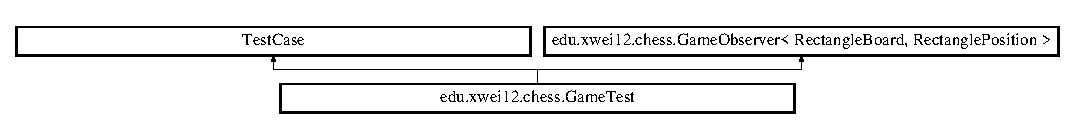
\includegraphics[height=1.290323cm]{classedu_1_1xwei12_1_1chess_1_1_game_test}
\end{center}
\end{figure}
\subsection*{Public Member Functions}
\begin{DoxyCompactItemize}
\item 
void {\bfseries set\+Up} ()  throws Exception \hypertarget{classedu_1_1xwei12_1_1chess_1_1_game_test_ab0d4d454595aa60d955e1988ad0d1d1a}{}\label{classedu_1_1xwei12_1_1chess_1_1_game_test_ab0d4d454595aa60d955e1988ad0d1d1a}

\item 
void {\bfseries test\+Step\+With\+Move} ()  throws Exception \hypertarget{classedu_1_1xwei12_1_1chess_1_1_game_test_a5d432efdcea691918b25c1f33d929038}{}\label{classedu_1_1xwei12_1_1chess_1_1_game_test_a5d432efdcea691918b25c1f33d929038}

\item 
void {\bfseries test\+Attack} ()  throws Exception \hypertarget{classedu_1_1xwei12_1_1chess_1_1_game_test_ad4361ea048b412a67e9b5dbcd5024561}{}\label{classedu_1_1xwei12_1_1chess_1_1_game_test_ad4361ea048b412a67e9b5dbcd5024561}

\item 
void {\bfseries test\+Checkmate} ()  throws Exception \hypertarget{classedu_1_1xwei12_1_1chess_1_1_game_test_a0e0dff24bd8370a9d82073629668b689}{}\label{classedu_1_1xwei12_1_1chess_1_1_game_test_a0e0dff24bd8370a9d82073629668b689}

\item 
void {\bfseries on\+Chess\+Game\+State\+Update} (\hyperlink{classedu_1_1xwei12_1_1chess_1_1_game}{Game}$<$ \hyperlink{classedu_1_1xwei12_1_1chess_1_1_rectangle_board}{Rectangle\+Board}, \hyperlink{classedu_1_1xwei12_1_1chess_1_1_rectangle_position}{Rectangle\+Position} $>$ game, \hyperlink{classedu_1_1xwei12_1_1chess_1_1_game}{Game}$<$ \hyperlink{classedu_1_1xwei12_1_1chess_1_1_rectangle_board}{Rectangle\+Board}, \hyperlink{classedu_1_1xwei12_1_1chess_1_1_rectangle_position}{Rectangle\+Position} $>$.Move move)\hypertarget{classedu_1_1xwei12_1_1chess_1_1_game_test_add5cdac8ecad3faeb4631f09cd333bd9}{}\label{classedu_1_1xwei12_1_1chess_1_1_game_test_add5cdac8ecad3faeb4631f09cd333bd9}

\end{DoxyCompactItemize}


\subsection{Detailed Description}
Created by xinranmsn on 2/4/16. 

The documentation for this class was generated from the following file\+:\begin{DoxyCompactItemize}
\item 
src/test/java/edu/xwei12/chess/Game\+Test.\+java\end{DoxyCompactItemize}

\hypertarget{classedu_1_1xwei12_1_1chess_1_1gui_1_1_g_u_i_test}{}\section{edu.\+xwei12.\+chess.\+gui.\+G\+U\+I\+Test Class Reference}
\label{classedu_1_1xwei12_1_1chess_1_1gui_1_1_g_u_i_test}\index{edu.\+xwei12.\+chess.\+gui.\+G\+U\+I\+Test@{edu.\+xwei12.\+chess.\+gui.\+G\+U\+I\+Test}}
\subsection*{Public Member Functions}
\begin{DoxyCompactItemize}
\item 
void {\bfseries set\+Up\+Class} ()  throws Interrupted\+Exception \hypertarget{classedu_1_1xwei12_1_1chess_1_1gui_1_1_g_u_i_test_a43357bf4e3193d4e9d250fa44ce43c8d}{}\label{classedu_1_1xwei12_1_1chess_1_1gui_1_1_g_u_i_test_a43357bf4e3193d4e9d250fa44ce43c8d}

\item 
void {\bfseries set\+Up} ()  throws Exception \hypertarget{classedu_1_1xwei12_1_1chess_1_1gui_1_1_g_u_i_test_ada470a6970547d07ae5d64fd76890a76}{}\label{classedu_1_1xwei12_1_1chess_1_1gui_1_1_g_u_i_test_ada470a6970547d07ae5d64fd76890a76}

\item 
void {\bfseries tear\+Down} ()  throws Exception \hypertarget{classedu_1_1xwei12_1_1chess_1_1gui_1_1_g_u_i_test_ad9b722cd977c3fcbe239345b6864ab0d}{}\label{classedu_1_1xwei12_1_1chess_1_1gui_1_1_g_u_i_test_ad9b722cd977c3fcbe239345b6864ab0d}

\item 
void {\bfseries test\+Start} ()  throws Exception \hypertarget{classedu_1_1xwei12_1_1chess_1_1gui_1_1_g_u_i_test_a0c0101bbf2cb04db0fcd467a24962750}{}\label{classedu_1_1xwei12_1_1chess_1_1gui_1_1_g_u_i_test_a0c0101bbf2cb04db0fcd467a24962750}

\end{DoxyCompactItemize}


\subsection{Detailed Description}
Test G\+UI \begin{DoxyAuthor}{Author}
Xinran Wei 
\end{DoxyAuthor}


The documentation for this class was generated from the following file\+:\begin{DoxyCompactItemize}
\item 
src/test/java/edu/xwei12/chess/gui/G\+U\+I\+Test.\+java\end{DoxyCompactItemize}

\hypertarget{classedu_1_1xwei12_1_1chess_1_1_game_1_1_move}{}\section{edu.\+xwei12.\+chess.\+Game$<$ B extends Board$<$ B, C, C extends Coordinates$<$ C $>$.Move Class Reference}
\label{classedu_1_1xwei12_1_1chess_1_1_game_1_1_move}\index{edu.\+xwei12.\+chess.\+Game$<$ B extends Board$<$ B, C, C extends Coordinates$<$ C $>$.\+Move@{edu.\+xwei12.\+chess.\+Game$<$ B extends Board$<$ B, C, C extends Coordinates$<$ C $>$.\+Move}}
\subsection*{Public Member Functions}
\begin{DoxyCompactItemize}
\item 
{\bfseries Move} (Integer player, C source, C destination)\hypertarget{classedu_1_1xwei12_1_1chess_1_1_game_1_1_move_ac15de338737674efff8defc8bde4687e}{}\label{classedu_1_1xwei12_1_1chess_1_1_game_1_1_move_ac15de338737674efff8defc8bde4687e}

\end{DoxyCompactItemize}
\subsection*{Public Attributes}
\begin{DoxyCompactItemize}
\item 
Integer {\bfseries player}\hypertarget{classedu_1_1xwei12_1_1chess_1_1_game_1_1_move_a8c7f161b862a49d80b0a8aa9d8a5aa30}{}\label{classedu_1_1xwei12_1_1chess_1_1_game_1_1_move_a8c7f161b862a49d80b0a8aa9d8a5aa30}

\item 
C {\bfseries source}\hypertarget{classedu_1_1xwei12_1_1chess_1_1_game_1_1_move_ab3afddeaccef45c7b93e7f7c82bf7952}{}\label{classedu_1_1xwei12_1_1chess_1_1_game_1_1_move_ab3afddeaccef45c7b93e7f7c82bf7952}

\item 
C {\bfseries destination}\hypertarget{classedu_1_1xwei12_1_1chess_1_1_game_1_1_move_a58ec0b87f29d223bb00e5d3a203fffd0}{}\label{classedu_1_1xwei12_1_1chess_1_1_game_1_1_move_a58ec0b87f29d223bb00e5d3a203fffd0}

\end{DoxyCompactItemize}


The documentation for this class was generated from the following file\+:\begin{DoxyCompactItemize}
\item 
src/main/java/edu/xwei12/chess/Game.\+java\end{DoxyCompactItemize}

\hypertarget{classedu_1_1xwei12_1_1chess_1_1_piece}{}\section{edu.\+xwei12.\+chess.\+Piece$<$ B extends Board, C extends Coordinates$<$ C $>$ Class Template Reference}
\label{classedu_1_1xwei12_1_1chess_1_1_piece}\index{edu.\+xwei12.\+chess.\+Piece$<$ B extends Board, C extends Coordinates$<$ C $>$@{edu.\+xwei12.\+chess.\+Piece$<$ B extends Board, C extends Coordinates$<$ C $>$}}
\subsection*{Classes}
\begin{DoxyCompactItemize}
\item 
interface {\bfseries Move\+Function}
\end{DoxyCompactItemize}
\subsection*{Public Member Functions}
\begin{DoxyCompactItemize}
\item 
String {\bfseries get\+Kind} ()\hypertarget{classedu_1_1xwei12_1_1chess_1_1_piece_a73b4aab85a136f4332ad2c5d8b381b85}{}\label{classedu_1_1xwei12_1_1chess_1_1_piece_a73b4aab85a136f4332ad2c5d8b381b85}

\item 
Integer {\bfseries get\+Tag} ()\hypertarget{classedu_1_1xwei12_1_1chess_1_1_piece_a4c66d1925435562706da902f6fd2e652}{}\label{classedu_1_1xwei12_1_1chess_1_1_piece_a4c66d1925435562706da902f6fd2e652}

\item 
\hyperlink{classedu_1_1xwei12_1_1chess_1_1_piece_acfd785e3c3cf8f00f1d0d7430b9e6f8b}{Piece} (String kind, int tag, Move\+Function$<$ B, C $>$ move\+Function)
\item 
Move\+Function$<$ B, C $>$ \hyperlink{classedu_1_1xwei12_1_1chess_1_1_piece_a12e3de9acb24ca9ff5e1f24c9e795075}{get\+Mover} ()
\end{DoxyCompactItemize}
\subsection*{Protected Member Functions}
\begin{DoxyCompactItemize}
\item 
void {\bfseries set\+Kind} (String kind)\hypertarget{classedu_1_1xwei12_1_1chess_1_1_piece_a1a1cd7f8732a010a052b4050b6d2b43f}{}\label{classedu_1_1xwei12_1_1chess_1_1_piece_a1a1cd7f8732a010a052b4050b6d2b43f}

\item 
void {\bfseries set\+Tag} (Integer tag)\hypertarget{classedu_1_1xwei12_1_1chess_1_1_piece_aecf345e53645feb46095e9199f056b09}{}\label{classedu_1_1xwei12_1_1chess_1_1_piece_aecf345e53645feb46095e9199f056b09}

\end{DoxyCompactItemize}


\subsection{Detailed Description}
\hyperlink{classedu_1_1xwei12_1_1chess_1_1_piece}{Piece} class \begin{DoxyAuthor}{Author}
Xinran Wei
\end{DoxyAuthor}
Properties\+: mover \+:\+: (position, board, distance) -\/$>$ position\+Set

The mover derives a set of possible moves (destination set) from the context (position, board cells, moving distance) 

\subsection{Constructor \& Destructor Documentation}
\index{edu\+::xwei12\+::chess\+::\+Piece@{edu\+::xwei12\+::chess\+::\+Piece}!Piece@{Piece}}
\index{Piece@{Piece}!edu\+::xwei12\+::chess\+::\+Piece@{edu\+::xwei12\+::chess\+::\+Piece}}
\subsubsection[{\texorpdfstring{Piece(\+String kind, int tag, Move\+Function$<$ B, C $>$ move\+Function)}{Piece(String kind, int tag, MoveFunction< B, C > moveFunction)}}]{\setlength{\rightskip}{0pt plus 5cm}{\bf edu.\+xwei12.\+chess.\+Piece}$<$ B extends {\bf Board}, C extends {\bf Coordinates}$<$ C $>$.{\bf Piece} (
\begin{DoxyParamCaption}
\item[{String}]{kind, }
\item[{int}]{tag, }
\item[{Move\+Function$<$ B, C $>$}]{move\+Function}
\end{DoxyParamCaption}
)\hspace{0.3cm}{\ttfamily [inline]}}\hypertarget{classedu_1_1xwei12_1_1chess_1_1_piece_acfd785e3c3cf8f00f1d0d7430b9e6f8b}{}\label{classedu_1_1xwei12_1_1chess_1_1_piece_acfd785e3c3cf8f00f1d0d7430b9e6f8b}
Constructor 
\begin{DoxyParams}{Parameters}
{\em move\+Function} & \+:\+: (position, board, distance) -\/$>$ position\+Set \\
\hline
\end{DoxyParams}


\subsection{Member Function Documentation}
\index{edu\+::xwei12\+::chess\+::\+Piece@{edu\+::xwei12\+::chess\+::\+Piece}!get\+Mover@{get\+Mover}}
\index{get\+Mover@{get\+Mover}!edu\+::xwei12\+::chess\+::\+Piece@{edu\+::xwei12\+::chess\+::\+Piece}}
\subsubsection[{\texorpdfstring{get\+Mover()}{getMover()}}]{\setlength{\rightskip}{0pt plus 5cm}Move\+Function$<$B, C$>$ {\bf edu.\+xwei12.\+chess.\+Piece}$<$ B extends {\bf Board}, C extends {\bf Coordinates}$<$ C $>$.get\+Mover (
\begin{DoxyParamCaption}
{}
\end{DoxyParamCaption}
)\hspace{0.3cm}{\ttfamily [inline]}}\hypertarget{classedu_1_1xwei12_1_1chess_1_1_piece_a12e3de9acb24ca9ff5e1f24c9e795075}{}\label{classedu_1_1xwei12_1_1chess_1_1_piece_a12e3de9acb24ca9ff5e1f24c9e795075}
Get move function \begin{DoxyReturn}{Returns}
Move function 
\end{DoxyReturn}


The documentation for this class was generated from the following file\+:\begin{DoxyCompactItemize}
\item 
src/main/java/edu/xwei12/chess/Piece.\+java\end{DoxyCompactItemize}

\hypertarget{classedu_1_1xwei12_1_1chess_1_1_piece_test}{}\section{edu.\+xwei12.\+chess.\+Piece\+Test Class Reference}
\label{classedu_1_1xwei12_1_1chess_1_1_piece_test}\index{edu.\+xwei12.\+chess.\+Piece\+Test@{edu.\+xwei12.\+chess.\+Piece\+Test}}
Inheritance diagram for edu.\+xwei12.\+chess.\+Piece\+Test\+:\begin{figure}[H]
\begin{center}
\leavevmode
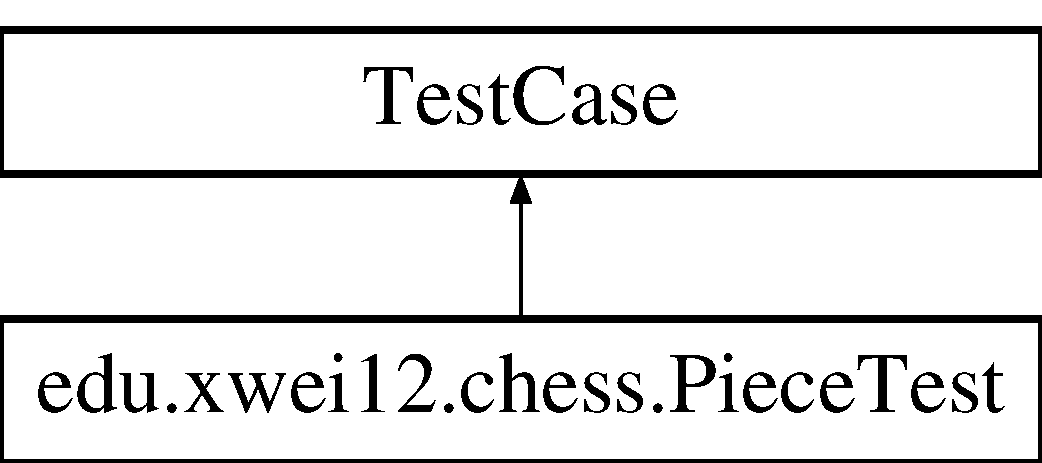
\includegraphics[height=2.000000cm]{classedu_1_1xwei12_1_1chess_1_1_piece_test}
\end{center}
\end{figure}
\subsection*{Public Member Functions}
\begin{DoxyCompactItemize}
\item 
void {\bfseries set\+Up} ()  throws Exception \hypertarget{classedu_1_1xwei12_1_1chess_1_1_piece_test_ab4b34267b3baa8a631b03b35910b3f49}{}\label{classedu_1_1xwei12_1_1chess_1_1_piece_test_ab4b34267b3baa8a631b03b35910b3f49}

\item 
void \hyperlink{classedu_1_1xwei12_1_1chess_1_1_piece_test_a2fe4db5ba7cfe46f6334ea4a68c3baa1}{test\+Pawn} ()  throws Exception 
\item 
void {\bfseries test\+Knight} ()  throws Exception \hypertarget{classedu_1_1xwei12_1_1chess_1_1_piece_test_a509a7e9086d76d4a91e92257a459b383}{}\label{classedu_1_1xwei12_1_1chess_1_1_piece_test_a509a7e9086d76d4a91e92257a459b383}

\item 
void {\bfseries test\+Rook} ()  throws Exception \hypertarget{classedu_1_1xwei12_1_1chess_1_1_piece_test_a69d5a7d273df11793c123411e7cc1ec1}{}\label{classedu_1_1xwei12_1_1chess_1_1_piece_test_a69d5a7d273df11793c123411e7cc1ec1}

\item 
void {\bfseries test\+Bishop} ()  throws Exception \hypertarget{classedu_1_1xwei12_1_1chess_1_1_piece_test_a274c5383772ca6cecdd3fb05ae6872a7}{}\label{classedu_1_1xwei12_1_1chess_1_1_piece_test_a274c5383772ca6cecdd3fb05ae6872a7}

\item 
void {\bfseries test\+King} ()  throws Exception \hypertarget{classedu_1_1xwei12_1_1chess_1_1_piece_test_a442cf194284606e1ba55b54a717a2175}{}\label{classedu_1_1xwei12_1_1chess_1_1_piece_test_a442cf194284606e1ba55b54a717a2175}

\item 
void {\bfseries test\+Grasshopper} ()  throws Exception \hypertarget{classedu_1_1xwei12_1_1chess_1_1_piece_test_ab6c983a0f322b35f75599027f1dbaffe}{}\label{classedu_1_1xwei12_1_1chess_1_1_piece_test_ab6c983a0f322b35f75599027f1dbaffe}

\item 
void {\bfseries test\+Beroline} ()  throws Exception \hypertarget{classedu_1_1xwei12_1_1chess_1_1_piece_test_ae0d535ce0bddc049078e5c2d71c6fb4d}{}\label{classedu_1_1xwei12_1_1chess_1_1_piece_test_ae0d535ce0bddc049078e5c2d71c6fb4d}

\end{DoxyCompactItemize}


\subsection{Detailed Description}
Created by xinranmsn on 2/4/16. 

\subsection{Member Function Documentation}
\index{edu\+::xwei12\+::chess\+::\+Piece\+Test@{edu\+::xwei12\+::chess\+::\+Piece\+Test}!test\+Pawn@{test\+Pawn}}
\index{test\+Pawn@{test\+Pawn}!edu\+::xwei12\+::chess\+::\+Piece\+Test@{edu\+::xwei12\+::chess\+::\+Piece\+Test}}
\subsubsection[{\texorpdfstring{test\+Pawn()}{testPawn()}}]{\setlength{\rightskip}{0pt plus 5cm}void edu.\+xwei12.\+chess.\+Piece\+Test.\+test\+Pawn (
\begin{DoxyParamCaption}
{}
\end{DoxyParamCaption}
) throws Exception\hspace{0.3cm}{\ttfamily [inline]}}\hypertarget{classedu_1_1xwei12_1_1chess_1_1_piece_test_a2fe4db5ba7cfe46f6334ea4a68c3baa1}{}\label{classedu_1_1xwei12_1_1chess_1_1_piece_test_a2fe4db5ba7cfe46f6334ea4a68c3baa1}
Default piece tests 

The documentation for this class was generated from the following file\+:\begin{DoxyCompactItemize}
\item 
src/test/java/edu/xwei12/chess/Piece\+Test.\+java\end{DoxyCompactItemize}

\hypertarget{classedu_1_1xwei12_1_1chess_1_1_rectangle_board}{}\section{edu.\+xwei12.\+chess.\+Rectangle\+Board Class Reference}
\label{classedu_1_1xwei12_1_1chess_1_1_rectangle_board}\index{edu.\+xwei12.\+chess.\+Rectangle\+Board@{edu.\+xwei12.\+chess.\+Rectangle\+Board}}
Inheritance diagram for edu.\+xwei12.\+chess.\+Rectangle\+Board\+:\begin{figure}[H]
\begin{center}
\leavevmode
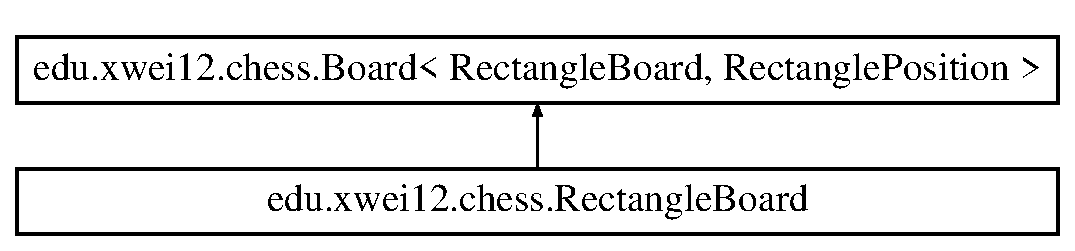
\includegraphics[height=2.000000cm]{classedu_1_1xwei12_1_1chess_1_1_rectangle_board}
\end{center}
\end{figure}
\subsection*{Public Member Functions}
\begin{DoxyCompactItemize}
\item 
int {\bfseries get\+Files} ()\hypertarget{classedu_1_1xwei12_1_1chess_1_1_rectangle_board_abb61689f6b76caa6caf8f5249b75fd78}{}\label{classedu_1_1xwei12_1_1chess_1_1_rectangle_board_abb61689f6b76caa6caf8f5249b75fd78}

\item 
int {\bfseries get\+Ranks} ()\hypertarget{classedu_1_1xwei12_1_1chess_1_1_rectangle_board_a85ea9a24fc63edc1cbcb077ea46f0ae3}{}\label{classedu_1_1xwei12_1_1chess_1_1_rectangle_board_a85ea9a24fc63edc1cbcb077ea46f0ae3}

\item 
\hyperlink{classedu_1_1xwei12_1_1chess_1_1_rectangle_board_a6406a4cfbabca7c41bcdcd9165764df0}{Rectangle\+Board} (int ranks, int files)
\item 
Set$<$ \hyperlink{classedu_1_1xwei12_1_1chess_1_1_rectangle_position}{Rectangle\+Position} $>$ \hyperlink{classedu_1_1xwei12_1_1chess_1_1_rectangle_board_a74cb08b9090a40990661e9283438d937}{get\+Pieces\+By\+Kind} (String kind)
\item 
Set$<$ String $>$ \hyperlink{classedu_1_1xwei12_1_1chess_1_1_rectangle_board_ab89613a1fa0c7178a6108a1ec7c3962b}{get\+All\+Piece\+Kinds} ()
\item 
boolean \hyperlink{classedu_1_1xwei12_1_1chess_1_1_rectangle_board_afd744749597e097cac2f9ab7abe7064d}{is\+Valid\+Position} (\hyperlink{classedu_1_1xwei12_1_1chess_1_1_rectangle_position}{Rectangle\+Position} position)
\item 
\hyperlink{classedu_1_1xwei12_1_1chess_1_1_piece}{Piece}$<$ \hyperlink{classedu_1_1xwei12_1_1chess_1_1_rectangle_board}{Rectangle\+Board}, \hyperlink{classedu_1_1xwei12_1_1chess_1_1_rectangle_position}{Rectangle\+Position} $>$ \hyperlink{classedu_1_1xwei12_1_1chess_1_1_rectangle_board_a4992efb221dfa1811e6b053ec91e3407}{get\+Piece} (\hyperlink{classedu_1_1xwei12_1_1chess_1_1_rectangle_position}{Rectangle\+Position} position)
\item 
void \hyperlink{classedu_1_1xwei12_1_1chess_1_1_rectangle_board_a629a12594a3edc1a33d88e4955591e48}{add\+Piece} (\hyperlink{classedu_1_1xwei12_1_1chess_1_1_piece}{Piece}$<$ \hyperlink{classedu_1_1xwei12_1_1chess_1_1_rectangle_board}{Rectangle\+Board}, \hyperlink{classedu_1_1xwei12_1_1chess_1_1_rectangle_position}{Rectangle\+Position} $>$ piece, \hyperlink{classedu_1_1xwei12_1_1chess_1_1_rectangle_position}{Rectangle\+Position} position)
\item 
Set$<$ \hyperlink{classedu_1_1xwei12_1_1chess_1_1_rectangle_position}{Rectangle\+Position} $>$ \hyperlink{classedu_1_1xwei12_1_1chess_1_1_rectangle_board_aebbe5e735c0759383c8407d964e1293e}{get\+Possible\+Moves} (\hyperlink{classedu_1_1xwei12_1_1chess_1_1_rectangle_position}{Rectangle\+Position} position, int distance)
\item 
boolean \hyperlink{classedu_1_1xwei12_1_1chess_1_1_rectangle_board_a65d288f3b314eb4efd80a85c95a556cd}{can\+Move\+Piece} (\hyperlink{classedu_1_1xwei12_1_1chess_1_1_rectangle_position}{Rectangle\+Position} from\+Position, \hyperlink{classedu_1_1xwei12_1_1chess_1_1_rectangle_position}{Rectangle\+Position} to\+Position)
\item 
boolean \hyperlink{classedu_1_1xwei12_1_1chess_1_1_rectangle_board_a476071ffa5222be6ea71f3fb82b7b8ff}{move\+Piece} (\hyperlink{classedu_1_1xwei12_1_1chess_1_1_rectangle_position}{Rectangle\+Position} from\+Position, \hyperlink{classedu_1_1xwei12_1_1chess_1_1_rectangle_position}{Rectangle\+Position} to\+Position)
\item 
int \hyperlink{classedu_1_1xwei12_1_1chess_1_1_rectangle_board_aeab8a752a9ea5b21569eff6decb53fd7}{leaps\+Needed} (\hyperlink{classedu_1_1xwei12_1_1chess_1_1_rectangle_position}{Rectangle\+Position} from\+Position, \hyperlink{classedu_1_1xwei12_1_1chess_1_1_rectangle_position}{Rectangle\+Position} to\+Position)
\item 
\hyperlink{classedu_1_1xwei12_1_1chess_1_1_rectangle_position}{Rectangle\+Position} \hyperlink{classedu_1_1xwei12_1_1chess_1_1_rectangle_board_ac0e3b5328b0ff0ac5dbc39688817da8c}{find\+Nearest\+Leap} (\hyperlink{classedu_1_1xwei12_1_1chess_1_1_rectangle_position}{Rectangle\+Position} from\+Position, \hyperlink{classedu_1_1xwei12_1_1chess_1_1_rectangle_position}{Rectangle\+Position} to\+Position)
\item 
void \hyperlink{classedu_1_1xwei12_1_1chess_1_1_rectangle_board_a2c0f4bdf89ab070895f93923774eb4ae}{print} ()
\end{DoxyCompactItemize}
\subsection*{Protected Member Functions}
\begin{DoxyCompactItemize}
\item 
\hyperlink{classedu_1_1xwei12_1_1chess_1_1_piece}{Piece}$<$ \hyperlink{classedu_1_1xwei12_1_1chess_1_1_rectangle_board}{Rectangle\+Board}, \hyperlink{classedu_1_1xwei12_1_1chess_1_1_rectangle_position}{Rectangle\+Position} $>$ \hyperlink{classedu_1_1xwei12_1_1chess_1_1_rectangle_board_a37e604e5a748f3d6fdeef458fb865049}{get\+Piece} (int rank, int file)
\end{DoxyCompactItemize}


\subsection{Detailed Description}
Chess board class \begin{DoxyAuthor}{Author}
Xinran Wei 
\end{DoxyAuthor}


\subsection{Constructor \& Destructor Documentation}
\index{edu\+::xwei12\+::chess\+::\+Rectangle\+Board@{edu\+::xwei12\+::chess\+::\+Rectangle\+Board}!Rectangle\+Board@{Rectangle\+Board}}
\index{Rectangle\+Board@{Rectangle\+Board}!edu\+::xwei12\+::chess\+::\+Rectangle\+Board@{edu\+::xwei12\+::chess\+::\+Rectangle\+Board}}
\subsubsection[{\texorpdfstring{Rectangle\+Board(int ranks, int files)}{RectangleBoard(int ranks, int files)}}]{\setlength{\rightskip}{0pt plus 5cm}edu.\+xwei12.\+chess.\+Rectangle\+Board.\+Rectangle\+Board (
\begin{DoxyParamCaption}
\item[{int}]{ranks, }
\item[{int}]{files}
\end{DoxyParamCaption}
)\hspace{0.3cm}{\ttfamily [inline]}}\hypertarget{classedu_1_1xwei12_1_1chess_1_1_rectangle_board_a6406a4cfbabca7c41bcdcd9165764df0}{}\label{classedu_1_1xwei12_1_1chess_1_1_rectangle_board_a6406a4cfbabca7c41bcdcd9165764df0}
Construct a board with dimensions 
\begin{DoxyParams}{Parameters}
{\em ranks} & number of ranks \\
\hline
{\em files} & number of files \\
\hline
\end{DoxyParams}


\subsection{Member Function Documentation}
\index{edu\+::xwei12\+::chess\+::\+Rectangle\+Board@{edu\+::xwei12\+::chess\+::\+Rectangle\+Board}!add\+Piece@{add\+Piece}}
\index{add\+Piece@{add\+Piece}!edu\+::xwei12\+::chess\+::\+Rectangle\+Board@{edu\+::xwei12\+::chess\+::\+Rectangle\+Board}}
\subsubsection[{\texorpdfstring{add\+Piece(\+Piece$<$ Rectangle\+Board, Rectangle\+Position $>$ piece, Rectangle\+Position position)}{addPiece(Piece< RectangleBoard, RectanglePosition > piece, RectanglePosition position)}}]{\setlength{\rightskip}{0pt plus 5cm}void edu.\+xwei12.\+chess.\+Rectangle\+Board.\+add\+Piece (
\begin{DoxyParamCaption}
\item[{{\bf Piece}$<$ {\bf Rectangle\+Board}, {\bf Rectangle\+Position} $>$}]{piece, }
\item[{{\bf Rectangle\+Position}}]{position}
\end{DoxyParamCaption}
)\hspace{0.3cm}{\ttfamily [inline]}}\hypertarget{classedu_1_1xwei12_1_1chess_1_1_rectangle_board_a629a12594a3edc1a33d88e4955591e48}{}\label{classedu_1_1xwei12_1_1chess_1_1_rectangle_board_a629a12594a3edc1a33d88e4955591e48}
Add a piece 
\begin{DoxyParams}{Parameters}
{\em piece} & a chess piece \\
\hline
{\em position} & position that the piece will be placed at \\
\hline
\end{DoxyParams}
\index{edu\+::xwei12\+::chess\+::\+Rectangle\+Board@{edu\+::xwei12\+::chess\+::\+Rectangle\+Board}!can\+Move\+Piece@{can\+Move\+Piece}}
\index{can\+Move\+Piece@{can\+Move\+Piece}!edu\+::xwei12\+::chess\+::\+Rectangle\+Board@{edu\+::xwei12\+::chess\+::\+Rectangle\+Board}}
\subsubsection[{\texorpdfstring{can\+Move\+Piece(\+Rectangle\+Position from\+Position, Rectangle\+Position to\+Position)}{canMovePiece(RectanglePosition fromPosition, RectanglePosition toPosition)}}]{\setlength{\rightskip}{0pt plus 5cm}boolean edu.\+xwei12.\+chess.\+Rectangle\+Board.\+can\+Move\+Piece (
\begin{DoxyParamCaption}
\item[{{\bf Rectangle\+Position}}]{from\+Position, }
\item[{{\bf Rectangle\+Position}}]{to\+Position}
\end{DoxyParamCaption}
)\hspace{0.3cm}{\ttfamily [inline]}}\hypertarget{classedu_1_1xwei12_1_1chess_1_1_rectangle_board_a65d288f3b314eb4efd80a85c95a556cd}{}\label{classedu_1_1xwei12_1_1chess_1_1_rectangle_board_a65d288f3b314eb4efd80a85c95a556cd}
Determine whether piece can be moved from a position to another 
\begin{DoxyParams}{Parameters}
{\em from\+Position} & source position \\
\hline
{\em to\+Position} & destination position \\
\hline
\end{DoxyParams}
\begin{DoxyReturn}{Returns}
can or can not 
\end{DoxyReturn}
\index{edu\+::xwei12\+::chess\+::\+Rectangle\+Board@{edu\+::xwei12\+::chess\+::\+Rectangle\+Board}!find\+Nearest\+Leap@{find\+Nearest\+Leap}}
\index{find\+Nearest\+Leap@{find\+Nearest\+Leap}!edu\+::xwei12\+::chess\+::\+Rectangle\+Board@{edu\+::xwei12\+::chess\+::\+Rectangle\+Board}}
\subsubsection[{\texorpdfstring{find\+Nearest\+Leap(\+Rectangle\+Position from\+Position, Rectangle\+Position to\+Position)}{findNearestLeap(RectanglePosition fromPosition, RectanglePosition toPosition)}}]{\setlength{\rightskip}{0pt plus 5cm}{\bf Rectangle\+Position} edu.\+xwei12.\+chess.\+Rectangle\+Board.\+find\+Nearest\+Leap (
\begin{DoxyParamCaption}
\item[{{\bf Rectangle\+Position}}]{from\+Position, }
\item[{{\bf Rectangle\+Position}}]{to\+Position}
\end{DoxyParamCaption}
)\hspace{0.3cm}{\ttfamily [inline]}}\hypertarget{classedu_1_1xwei12_1_1chess_1_1_rectangle_board_ac0e3b5328b0ff0ac5dbc39688817da8c}{}\label{classedu_1_1xwei12_1_1chess_1_1_rectangle_board_ac0e3b5328b0ff0ac5dbc39688817da8c}
Find the first leap from source to destination. 
\begin{DoxyParams}{Parameters}
{\em from\+Position} & source position \\
\hline
{\em to\+Position} & destination position \\
\hline
\end{DoxyParams}
\begin{DoxyReturn}{Returns}
position of the leap or null 
\end{DoxyReturn}
\index{edu\+::xwei12\+::chess\+::\+Rectangle\+Board@{edu\+::xwei12\+::chess\+::\+Rectangle\+Board}!get\+All\+Piece\+Kinds@{get\+All\+Piece\+Kinds}}
\index{get\+All\+Piece\+Kinds@{get\+All\+Piece\+Kinds}!edu\+::xwei12\+::chess\+::\+Rectangle\+Board@{edu\+::xwei12\+::chess\+::\+Rectangle\+Board}}
\subsubsection[{\texorpdfstring{get\+All\+Piece\+Kinds()}{getAllPieceKinds()}}]{\setlength{\rightskip}{0pt plus 5cm}Set$<$String$>$ edu.\+xwei12.\+chess.\+Rectangle\+Board.\+get\+All\+Piece\+Kinds (
\begin{DoxyParamCaption}
{}
\end{DoxyParamCaption}
)\hspace{0.3cm}{\ttfamily [inline]}}\hypertarget{classedu_1_1xwei12_1_1chess_1_1_rectangle_board_ab89613a1fa0c7178a6108a1ec7c3962b}{}\label{classedu_1_1xwei12_1_1chess_1_1_rectangle_board_ab89613a1fa0c7178a6108a1ec7c3962b}
Get all piece names \begin{DoxyReturn}{Returns}
all kinds of pieces, such as \{\char`\"{}pawn\char`\"{}, \char`\"{}king\char`\"{}, ...\} 
\end{DoxyReturn}
\index{edu\+::xwei12\+::chess\+::\+Rectangle\+Board@{edu\+::xwei12\+::chess\+::\+Rectangle\+Board}!get\+Piece@{get\+Piece}}
\index{get\+Piece@{get\+Piece}!edu\+::xwei12\+::chess\+::\+Rectangle\+Board@{edu\+::xwei12\+::chess\+::\+Rectangle\+Board}}
\subsubsection[{\texorpdfstring{get\+Piece(int rank, int file)}{getPiece(int rank, int file)}}]{\setlength{\rightskip}{0pt plus 5cm}{\bf Piece}$<${\bf Rectangle\+Board}, {\bf Rectangle\+Position}$>$ edu.\+xwei12.\+chess.\+Rectangle\+Board.\+get\+Piece (
\begin{DoxyParamCaption}
\item[{int}]{rank, }
\item[{int}]{file}
\end{DoxyParamCaption}
)\hspace{0.3cm}{\ttfamily [inline]}, {\ttfamily [protected]}}\hypertarget{classedu_1_1xwei12_1_1chess_1_1_rectangle_board_a37e604e5a748f3d6fdeef458fb865049}{}\label{classedu_1_1xwei12_1_1chess_1_1_rectangle_board_a37e604e5a748f3d6fdeef458fb865049}
Get piece at (rank, file) 
\begin{DoxyParams}{Parameters}
{\em rank} & rank-\/coordinate \\
\hline
{\em file} & file-\/coordinate \\
\hline
\end{DoxyParams}
\begin{DoxyReturn}{Returns}
cell 
\end{DoxyReturn}
\index{edu\+::xwei12\+::chess\+::\+Rectangle\+Board@{edu\+::xwei12\+::chess\+::\+Rectangle\+Board}!get\+Piece@{get\+Piece}}
\index{get\+Piece@{get\+Piece}!edu\+::xwei12\+::chess\+::\+Rectangle\+Board@{edu\+::xwei12\+::chess\+::\+Rectangle\+Board}}
\subsubsection[{\texorpdfstring{get\+Piece(\+Rectangle\+Position position)}{getPiece(RectanglePosition position)}}]{\setlength{\rightskip}{0pt plus 5cm}{\bf Piece}$<${\bf Rectangle\+Board}, {\bf Rectangle\+Position}$>$ edu.\+xwei12.\+chess.\+Rectangle\+Board.\+get\+Piece (
\begin{DoxyParamCaption}
\item[{{\bf Rectangle\+Position}}]{position}
\end{DoxyParamCaption}
)\hspace{0.3cm}{\ttfamily [inline]}}\hypertarget{classedu_1_1xwei12_1_1chess_1_1_rectangle_board_a4992efb221dfa1811e6b053ec91e3407}{}\label{classedu_1_1xwei12_1_1chess_1_1_rectangle_board_a4992efb221dfa1811e6b053ec91e3407}
\hyperlink{classedu_1_1xwei12_1_1chess_1_1_piece}{Piece} at position 
\begin{DoxyParams}{Parameters}
{\em position} & position of the piece, dependent on the coordinate system (\hyperlink{interfaceedu_1_1xwei12_1_1chess_1_1_coordinates}{Coordinates}) \\
\hline
\end{DoxyParams}
\begin{DoxyReturn}{Returns}
piece or null 
\end{DoxyReturn}
\index{edu\+::xwei12\+::chess\+::\+Rectangle\+Board@{edu\+::xwei12\+::chess\+::\+Rectangle\+Board}!get\+Pieces\+By\+Kind@{get\+Pieces\+By\+Kind}}
\index{get\+Pieces\+By\+Kind@{get\+Pieces\+By\+Kind}!edu\+::xwei12\+::chess\+::\+Rectangle\+Board@{edu\+::xwei12\+::chess\+::\+Rectangle\+Board}}
\subsubsection[{\texorpdfstring{get\+Pieces\+By\+Kind(\+String kind)}{getPiecesByKind(String kind)}}]{\setlength{\rightskip}{0pt plus 5cm}Set$<${\bf Rectangle\+Position}$>$ edu.\+xwei12.\+chess.\+Rectangle\+Board.\+get\+Pieces\+By\+Kind (
\begin{DoxyParamCaption}
\item[{String}]{kind}
\end{DoxyParamCaption}
)\hspace{0.3cm}{\ttfamily [inline]}}\hypertarget{classedu_1_1xwei12_1_1chess_1_1_rectangle_board_a74cb08b9090a40990661e9283438d937}{}\label{classedu_1_1xwei12_1_1chess_1_1_rectangle_board_a74cb08b9090a40990661e9283438d937}
Get locations of pieces of a kind 
\begin{DoxyParams}{Parameters}
{\em kind} & name of the kind \\
\hline
\end{DoxyParams}
\begin{DoxyReturn}{Returns}
piece set 
\end{DoxyReturn}
\index{edu\+::xwei12\+::chess\+::\+Rectangle\+Board@{edu\+::xwei12\+::chess\+::\+Rectangle\+Board}!get\+Possible\+Moves@{get\+Possible\+Moves}}
\index{get\+Possible\+Moves@{get\+Possible\+Moves}!edu\+::xwei12\+::chess\+::\+Rectangle\+Board@{edu\+::xwei12\+::chess\+::\+Rectangle\+Board}}
\subsubsection[{\texorpdfstring{get\+Possible\+Moves(\+Rectangle\+Position position, int distance)}{getPossibleMoves(RectanglePosition position, int distance)}}]{\setlength{\rightskip}{0pt plus 5cm}Set$<${\bf Rectangle\+Position}$>$ edu.\+xwei12.\+chess.\+Rectangle\+Board.\+get\+Possible\+Moves (
\begin{DoxyParamCaption}
\item[{{\bf Rectangle\+Position}}]{position, }
\item[{int}]{distance}
\end{DoxyParamCaption}
)\hspace{0.3cm}{\ttfamily [inline]}}\hypertarget{classedu_1_1xwei12_1_1chess_1_1_rectangle_board_aebbe5e735c0759383c8407d964e1293e}{}\label{classedu_1_1xwei12_1_1chess_1_1_rectangle_board_aebbe5e735c0759383c8407d964e1293e}
Get a set of possible moves at distance for the piece at position 
\begin{DoxyParams}{Parameters}
{\em position} & source position \\
\hline
{\em distance} & distance of move \\
\hline
\end{DoxyParams}
\begin{DoxyReturn}{Returns}
position set 
\end{DoxyReturn}
\index{edu\+::xwei12\+::chess\+::\+Rectangle\+Board@{edu\+::xwei12\+::chess\+::\+Rectangle\+Board}!is\+Valid\+Position@{is\+Valid\+Position}}
\index{is\+Valid\+Position@{is\+Valid\+Position}!edu\+::xwei12\+::chess\+::\+Rectangle\+Board@{edu\+::xwei12\+::chess\+::\+Rectangle\+Board}}
\subsubsection[{\texorpdfstring{is\+Valid\+Position(\+Rectangle\+Position position)}{isValidPosition(RectanglePosition position)}}]{\setlength{\rightskip}{0pt plus 5cm}boolean edu.\+xwei12.\+chess.\+Rectangle\+Board.\+is\+Valid\+Position (
\begin{DoxyParamCaption}
\item[{{\bf Rectangle\+Position}}]{position}
\end{DoxyParamCaption}
)\hspace{0.3cm}{\ttfamily [inline]}}\hypertarget{classedu_1_1xwei12_1_1chess_1_1_rectangle_board_afd744749597e097cac2f9ab7abe7064d}{}\label{classedu_1_1xwei12_1_1chess_1_1_rectangle_board_afd744749597e097cac2f9ab7abe7064d}
Determines if a position is on the board 
\begin{DoxyParams}{Parameters}
{\em position} & position \\
\hline
\end{DoxyParams}
\begin{DoxyReturn}{Returns}
valid or not 
\end{DoxyReturn}
\index{edu\+::xwei12\+::chess\+::\+Rectangle\+Board@{edu\+::xwei12\+::chess\+::\+Rectangle\+Board}!leaps\+Needed@{leaps\+Needed}}
\index{leaps\+Needed@{leaps\+Needed}!edu\+::xwei12\+::chess\+::\+Rectangle\+Board@{edu\+::xwei12\+::chess\+::\+Rectangle\+Board}}
\subsubsection[{\texorpdfstring{leaps\+Needed(\+Rectangle\+Position from\+Position, Rectangle\+Position to\+Position)}{leapsNeeded(RectanglePosition fromPosition, RectanglePosition toPosition)}}]{\setlength{\rightskip}{0pt plus 5cm}int edu.\+xwei12.\+chess.\+Rectangle\+Board.\+leaps\+Needed (
\begin{DoxyParamCaption}
\item[{{\bf Rectangle\+Position}}]{from\+Position, }
\item[{{\bf Rectangle\+Position}}]{to\+Position}
\end{DoxyParamCaption}
)\hspace{0.3cm}{\ttfamily [inline]}}\hypertarget{classedu_1_1xwei12_1_1chess_1_1_rectangle_board_aeab8a752a9ea5b21569eff6decb53fd7}{}\label{classedu_1_1xwei12_1_1chess_1_1_rectangle_board_aeab8a752a9ea5b21569eff6decb53fd7}
Determine whether there\textquotesingle{}s any piece blocking the path from source to destination, i.\+e., whether a leap is needed 
\begin{DoxyParams}{Parameters}
{\em from\+Position} & source position \\
\hline
{\em to\+Position} & destination position \\
\hline
\end{DoxyParams}
\begin{DoxyReturn}{Returns}
number of leaps needed 
\end{DoxyReturn}
\index{edu\+::xwei12\+::chess\+::\+Rectangle\+Board@{edu\+::xwei12\+::chess\+::\+Rectangle\+Board}!move\+Piece@{move\+Piece}}
\index{move\+Piece@{move\+Piece}!edu\+::xwei12\+::chess\+::\+Rectangle\+Board@{edu\+::xwei12\+::chess\+::\+Rectangle\+Board}}
\subsubsection[{\texorpdfstring{move\+Piece(\+Rectangle\+Position from\+Position, Rectangle\+Position to\+Position)}{movePiece(RectanglePosition fromPosition, RectanglePosition toPosition)}}]{\setlength{\rightskip}{0pt plus 5cm}boolean edu.\+xwei12.\+chess.\+Rectangle\+Board.\+move\+Piece (
\begin{DoxyParamCaption}
\item[{{\bf Rectangle\+Position}}]{from\+Position, }
\item[{{\bf Rectangle\+Position}}]{to\+Position}
\end{DoxyParamCaption}
)\hspace{0.3cm}{\ttfamily [inline]}}\hypertarget{classedu_1_1xwei12_1_1chess_1_1_rectangle_board_a476071ffa5222be6ea71f3fb82b7b8ff}{}\label{classedu_1_1xwei12_1_1chess_1_1_rectangle_board_a476071ffa5222be6ea71f3fb82b7b8ff}
Move a piece from one position to another, and also attacks 
\begin{DoxyParams}{Parameters}
{\em from\+Position} & current position of piece \\
\hline
{\em to\+Position} & of movement \\
\hline
\end{DoxyParams}
\begin{DoxyReturn}{Returns}
success 
\end{DoxyReturn}
\index{edu\+::xwei12\+::chess\+::\+Rectangle\+Board@{edu\+::xwei12\+::chess\+::\+Rectangle\+Board}!print@{print}}
\index{print@{print}!edu\+::xwei12\+::chess\+::\+Rectangle\+Board@{edu\+::xwei12\+::chess\+::\+Rectangle\+Board}}
\subsubsection[{\texorpdfstring{print()}{print()}}]{\setlength{\rightskip}{0pt plus 5cm}void edu.\+xwei12.\+chess.\+Rectangle\+Board.\+print (
\begin{DoxyParamCaption}
{}
\end{DoxyParamCaption}
)\hspace{0.3cm}{\ttfamily [inline]}}\hypertarget{classedu_1_1xwei12_1_1chess_1_1_rectangle_board_a2c0f4bdf89ab070895f93923774eb4ae}{}\label{classedu_1_1xwei12_1_1chess_1_1_rectangle_board_a2c0f4bdf89ab070895f93923774eb4ae}
Print chess board (helper) 

The documentation for this class was generated from the following file\+:\begin{DoxyCompactItemize}
\item 
src/main/java/edu/xwei12/chess/Rectangle\+Board.\+java\end{DoxyCompactItemize}

\hypertarget{classedu_1_1xwei12_1_1chess_1_1_rectangle_position}{}\section{edu.\+xwei12.\+chess.\+Rectangle\+Position Class Reference}
\label{classedu_1_1xwei12_1_1chess_1_1_rectangle_position}\index{edu.\+xwei12.\+chess.\+Rectangle\+Position@{edu.\+xwei12.\+chess.\+Rectangle\+Position}}
Inheritance diagram for edu.\+xwei12.\+chess.\+Rectangle\+Position\+:\begin{figure}[H]
\begin{center}
\leavevmode
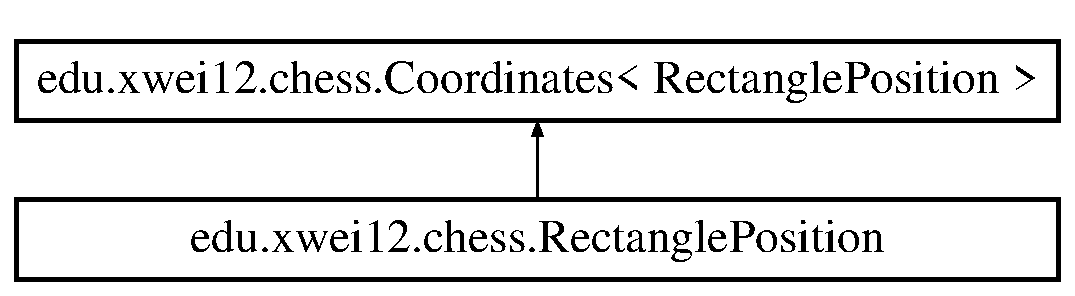
\includegraphics[height=2.000000cm]{classedu_1_1xwei12_1_1chess_1_1_rectangle_position}
\end{center}
\end{figure}
\subsection*{Public Member Functions}
\begin{DoxyCompactItemize}
\item 
\hyperlink{classedu_1_1xwei12_1_1chess_1_1_rectangle_position_ab72fff693d3435a30423cd307860e44c}{Rectangle\+Position} (int \hyperlink{classedu_1_1xwei12_1_1chess_1_1_rectangle_position_a6dd9047eb4002335ba2ad44621ca3407}{rank}, int \hyperlink{classedu_1_1xwei12_1_1chess_1_1_rectangle_position_ac7e18a9bb18f8a1d2ef0b6591fa4bffd}{file})
\item 
int \hyperlink{classedu_1_1xwei12_1_1chess_1_1_rectangle_position_a32ae95db005f0f4776ec8cc9c474da25}{distance\+To} (\hyperlink{classedu_1_1xwei12_1_1chess_1_1_rectangle_position}{Rectangle\+Position} destination)
\item 
boolean \hyperlink{classedu_1_1xwei12_1_1chess_1_1_rectangle_position_a2f1d3536238edecb82e98b60f7d5b52e}{same\+As} (\hyperlink{classedu_1_1xwei12_1_1chess_1_1_rectangle_position}{Rectangle\+Position} other)
\end{DoxyCompactItemize}
\subsection*{Public Attributes}
\begin{DoxyCompactItemize}
\item 
int \hyperlink{classedu_1_1xwei12_1_1chess_1_1_rectangle_position_a6dd9047eb4002335ba2ad44621ca3407}{rank}
\item 
int \hyperlink{classedu_1_1xwei12_1_1chess_1_1_rectangle_position_ac7e18a9bb18f8a1d2ef0b6591fa4bffd}{file}
\end{DoxyCompactItemize}


\subsection{Detailed Description}
Rectangle coordinate system \begin{DoxyAuthor}{Author}
Xinran Wei 
\end{DoxyAuthor}


\subsection{Constructor \& Destructor Documentation}
\index{edu\+::xwei12\+::chess\+::\+Rectangle\+Position@{edu\+::xwei12\+::chess\+::\+Rectangle\+Position}!Rectangle\+Position@{Rectangle\+Position}}
\index{Rectangle\+Position@{Rectangle\+Position}!edu\+::xwei12\+::chess\+::\+Rectangle\+Position@{edu\+::xwei12\+::chess\+::\+Rectangle\+Position}}
\subsubsection[{\texorpdfstring{Rectangle\+Position(int rank, int file)}{RectanglePosition(int rank, int file)}}]{\setlength{\rightskip}{0pt plus 5cm}edu.\+xwei12.\+chess.\+Rectangle\+Position.\+Rectangle\+Position (
\begin{DoxyParamCaption}
\item[{int}]{rank, }
\item[{int}]{file}
\end{DoxyParamCaption}
)\hspace{0.3cm}{\ttfamily [inline]}}\hypertarget{classedu_1_1xwei12_1_1chess_1_1_rectangle_position_ab72fff693d3435a30423cd307860e44c}{}\label{classedu_1_1xwei12_1_1chess_1_1_rectangle_position_ab72fff693d3435a30423cd307860e44c}
Constructor of coordinates 
\begin{DoxyParams}{Parameters}
{\em rank} & rank-\/coordinate \\
\hline
{\em file} & file-\/coordinate \\
\hline
\end{DoxyParams}


\subsection{Member Function Documentation}
\index{edu\+::xwei12\+::chess\+::\+Rectangle\+Position@{edu\+::xwei12\+::chess\+::\+Rectangle\+Position}!distance\+To@{distance\+To}}
\index{distance\+To@{distance\+To}!edu\+::xwei12\+::chess\+::\+Rectangle\+Position@{edu\+::xwei12\+::chess\+::\+Rectangle\+Position}}
\subsubsection[{\texorpdfstring{distance\+To(\+Rectangle\+Position destination)}{distanceTo(RectanglePosition destination)}}]{\setlength{\rightskip}{0pt plus 5cm}int edu.\+xwei12.\+chess.\+Rectangle\+Position.\+distance\+To (
\begin{DoxyParamCaption}
\item[{{\bf Rectangle\+Position}}]{destination}
\end{DoxyParamCaption}
)\hspace{0.3cm}{\ttfamily [inline]}}\hypertarget{classedu_1_1xwei12_1_1chess_1_1_rectangle_position_a32ae95db005f0f4776ec8cc9c474da25}{}\label{classedu_1_1xwei12_1_1chess_1_1_rectangle_position_a32ae95db005f0f4776ec8cc9c474da25}
Compute distance from self to another 
\begin{DoxyParams}{Parameters}
{\em destination} & destination position \\
\hline
\end{DoxyParams}
\begin{DoxyReturn}{Returns}
distance 
\end{DoxyReturn}
\index{edu\+::xwei12\+::chess\+::\+Rectangle\+Position@{edu\+::xwei12\+::chess\+::\+Rectangle\+Position}!same\+As@{same\+As}}
\index{same\+As@{same\+As}!edu\+::xwei12\+::chess\+::\+Rectangle\+Position@{edu\+::xwei12\+::chess\+::\+Rectangle\+Position}}
\subsubsection[{\texorpdfstring{same\+As(\+Rectangle\+Position other)}{sameAs(RectanglePosition other)}}]{\setlength{\rightskip}{0pt plus 5cm}boolean edu.\+xwei12.\+chess.\+Rectangle\+Position.\+same\+As (
\begin{DoxyParamCaption}
\item[{{\bf Rectangle\+Position}}]{other}
\end{DoxyParamCaption}
)\hspace{0.3cm}{\ttfamily [inline]}}\hypertarget{classedu_1_1xwei12_1_1chess_1_1_rectangle_position_a2f1d3536238edecb82e98b60f7d5b52e}{}\label{classedu_1_1xwei12_1_1chess_1_1_rectangle_position_a2f1d3536238edecb82e98b60f7d5b52e}
Determine whether self is the same as other 
\begin{DoxyParams}{Parameters}
{\em other} & the other position \\
\hline
\end{DoxyParams}
\begin{DoxyReturn}{Returns}
equals or not 
\end{DoxyReturn}


\subsection{Member Data Documentation}
\index{edu\+::xwei12\+::chess\+::\+Rectangle\+Position@{edu\+::xwei12\+::chess\+::\+Rectangle\+Position}!file@{file}}
\index{file@{file}!edu\+::xwei12\+::chess\+::\+Rectangle\+Position@{edu\+::xwei12\+::chess\+::\+Rectangle\+Position}}
\subsubsection[{\texorpdfstring{file}{file}}]{\setlength{\rightskip}{0pt plus 5cm}int edu.\+xwei12.\+chess.\+Rectangle\+Position.\+file}\hypertarget{classedu_1_1xwei12_1_1chess_1_1_rectangle_position_ac7e18a9bb18f8a1d2ef0b6591fa4bffd}{}\label{classedu_1_1xwei12_1_1chess_1_1_rectangle_position_ac7e18a9bb18f8a1d2ef0b6591fa4bffd}
File component of the coordinates \index{edu\+::xwei12\+::chess\+::\+Rectangle\+Position@{edu\+::xwei12\+::chess\+::\+Rectangle\+Position}!rank@{rank}}
\index{rank@{rank}!edu\+::xwei12\+::chess\+::\+Rectangle\+Position@{edu\+::xwei12\+::chess\+::\+Rectangle\+Position}}
\subsubsection[{\texorpdfstring{rank}{rank}}]{\setlength{\rightskip}{0pt plus 5cm}int edu.\+xwei12.\+chess.\+Rectangle\+Position.\+rank}\hypertarget{classedu_1_1xwei12_1_1chess_1_1_rectangle_position_a6dd9047eb4002335ba2ad44621ca3407}{}\label{classedu_1_1xwei12_1_1chess_1_1_rectangle_position_a6dd9047eb4002335ba2ad44621ca3407}
Rank component of the coordinates 

The documentation for this class was generated from the following file\+:\begin{DoxyCompactItemize}
\item 
src/main/java/edu/xwei12/chess/Rectangle\+Position.\+java\end{DoxyCompactItemize}

\hypertarget{classedu_1_1xwei12_1_1chess_1_1_standard_game}{}\section{edu.\+xwei12.\+chess.\+Standard\+Game Class Reference}
\label{classedu_1_1xwei12_1_1chess_1_1_standard_game}\index{edu.\+xwei12.\+chess.\+Standard\+Game@{edu.\+xwei12.\+chess.\+Standard\+Game}}
Inheritance diagram for edu.\+xwei12.\+chess.\+Standard\+Game\+:\begin{figure}[H]
\begin{center}
\leavevmode
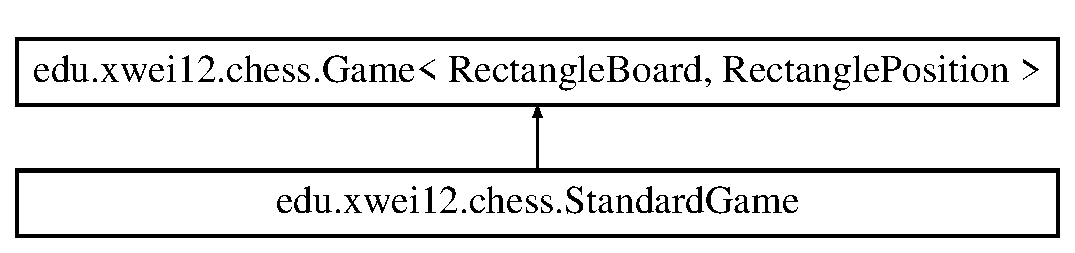
\includegraphics[height=2.000000cm]{classedu_1_1xwei12_1_1chess_1_1_standard_game}
\end{center}
\end{figure}
\subsection*{Public Member Functions}
\begin{DoxyCompactItemize}
\item 
boolean \hyperlink{classedu_1_1xwei12_1_1chess_1_1_standard_game_a12bb21a8f25e113d1775be551edde233}{step\+With\+Move} (Integer player, int fromX, int fromY, int toX, int toY)
\end{DoxyCompactItemize}
\subsection*{Static Public Attributes}
\begin{DoxyCompactItemize}
\item 
static final int {\bfseries P\+L\+A\+Y\+E\+R\+\_\+A} = 1\hypertarget{classedu_1_1xwei12_1_1chess_1_1_standard_game_a1ce97a54be76cb25b9d1f2c6ade8d974}{}\label{classedu_1_1xwei12_1_1chess_1_1_standard_game_a1ce97a54be76cb25b9d1f2c6ade8d974}

\item 
static final int {\bfseries P\+L\+A\+Y\+E\+R\+\_\+B} = -\/1\hypertarget{classedu_1_1xwei12_1_1chess_1_1_standard_game_ada025f7928a6e9d12fda509072851e22}{}\label{classedu_1_1xwei12_1_1chess_1_1_standard_game_ada025f7928a6e9d12fda509072851e22}

\end{DoxyCompactItemize}
\subsection*{Additional Inherited Members}


\subsection{Detailed Description}
Standard rectangle game \begin{DoxyAuthor}{Author}
Xinran Wei 
\end{DoxyAuthor}


\subsection{Member Function Documentation}
\index{edu\+::xwei12\+::chess\+::\+Standard\+Game@{edu\+::xwei12\+::chess\+::\+Standard\+Game}!step\+With\+Move@{step\+With\+Move}}
\index{step\+With\+Move@{step\+With\+Move}!edu\+::xwei12\+::chess\+::\+Standard\+Game@{edu\+::xwei12\+::chess\+::\+Standard\+Game}}
\subsubsection[{\texorpdfstring{step\+With\+Move(\+Integer player, int from\+X, int from\+Y, int to\+X, int to\+Y)}{stepWithMove(Integer player, int fromX, int fromY, int toX, int toY)}}]{\setlength{\rightskip}{0pt plus 5cm}boolean edu.\+xwei12.\+chess.\+Standard\+Game.\+step\+With\+Move (
\begin{DoxyParamCaption}
\item[{Integer}]{player, }
\item[{int}]{fromX, }
\item[{int}]{fromY, }
\item[{int}]{toX, }
\item[{int}]{toY}
\end{DoxyParamCaption}
)\hspace{0.3cm}{\ttfamily [inline]}}\hypertarget{classedu_1_1xwei12_1_1chess_1_1_standard_game_a12bb21a8f25e113d1775be551edde233}{}\label{classedu_1_1xwei12_1_1chess_1_1_standard_game_a12bb21a8f25e113d1775be551edde233}
Stepping helper with rectangle coordinates 
\begin{DoxyParams}{Parameters}
{\em player} & player tag \\
\hline
{\em fromX} & source rank-\/coordinate \\
\hline
{\em fromY} & source file-\/coordinate \\
\hline
{\em toX} & destination rank-\/coordinate \\
\hline
{\em toY} & destination file-\/coordinate \\
\hline
\end{DoxyParams}
\begin{DoxyReturn}{Returns}
moved 
\end{DoxyReturn}


The documentation for this class was generated from the following file\+:\begin{DoxyCompactItemize}
\item 
src/main/java/edu/xwei12/chess/Standard\+Game.\+java\end{DoxyCompactItemize}

\hypertarget{enumedu_1_1xwei12_1_1chess_1_1_game_1_1_state}{}\section{edu.\+xwei12.\+chess.\+Game$<$ B extends Board$<$ B, C, C extends Coordinates$<$ C $>$.State Enum Reference}
\label{enumedu_1_1xwei12_1_1chess_1_1_game_1_1_state}\index{edu.\+xwei12.\+chess.\+Game$<$ B extends Board$<$ B, C, C extends Coordinates$<$ C $>$.\+State@{edu.\+xwei12.\+chess.\+Game$<$ B extends Board$<$ B, C, C extends Coordinates$<$ C $>$.\+State}}
\subsection*{Public Attributes}
\begin{DoxyCompactItemize}
\item 
{\bfseries N\+O\+R\+M\+AL}\hypertarget{enumedu_1_1xwei12_1_1chess_1_1_game_1_1_state_a6c56bbb3d917ac45c9420b5e3dace42d}{}\label{enumedu_1_1xwei12_1_1chess_1_1_game_1_1_state_a6c56bbb3d917ac45c9420b5e3dace42d}

\item 
{\bfseries C\+H\+E\+C\+K\+M\+A\+TE}\hypertarget{enumedu_1_1xwei12_1_1chess_1_1_game_1_1_state_abcbb442bcc94baa4d8b807e9dbb7f3eb}{}\label{enumedu_1_1xwei12_1_1chess_1_1_game_1_1_state_abcbb442bcc94baa4d8b807e9dbb7f3eb}

\end{DoxyCompactItemize}


The documentation for this enum was generated from the following file\+:\begin{DoxyCompactItemize}
\item 
src/main/java/edu/xwei12/chess/Game.\+java\end{DoxyCompactItemize}

%--- End generated contents ---

% Index
\backmatter
\newpage
\phantomsection
\clearemptydoublepage
\addcontentsline{toc}{chapter}{Index}
\printindex

\end{document}
